\documentclass[11pt]{article}

% Change "review" to "final" to generate the final (sometimes called camera-ready) version.
% Change to "preprint" to generate a non-anonymous version with page numbers.
%\usepackage[review]{acl}
\usepackage[preprint]{acl}

% Standard package includes
\usepackage{times}
\usepackage{latexsym}

% For proper rendering and hyphenation of words containing Latin characters (including in bib files)
\usepackage[T1]{fontenc}
% For Vietnamese characters
% \usepackage[T5]{fontenc}
% See https://www.latex-project.org/help/documentation/encguide.pdf for other character sets

% This assumes your files are encoded as UTF8
\usepackage[utf8]{inputenc}

% This is not strictly necessary, and may be commented out,
% but it will improve the layout of the manuscript,
% and will typically save some space.
\usepackage{microtype}

% This is also not strictly necessary, and may be commented out.
% However, it will improve the aesthetics of text in
% the typewriter font.
\usepackage{inconsolata}

%Including images in your LaTeX document requires adding
%additional package(s)
\usepackage{graphicx}
\usepackage{multirow}
\usepackage[T1]{fontenc}    % use 8-bit T1 fonts
\usepackage{url}            % simple URL typesetting
\usepackage{hyperref}       % hyperlinks
\hypersetup{breaklinks=true}
\usepackage{booktabs}       % professional-quality tables
\usepackage{amsfonts}       % blackboard math symbols
\usepackage{nicefrac}       % compact symbols for 1/2, etc.
\usepackage{microtype}      % microtypography
\usepackage{xcolor}         % colors
\usepackage[table]{xcolor}
% \usepackage{natbib}
\usepackage{graphicx}
\usepackage{subcaption}
\usepackage{placeins}

%% For the appendix
%\usepackage[most]{tcolorbox} commented out
\usepackage{listings}
\usepackage{float}
%\usepackage{todonotes} commented out
\usepackage{array} % for better column types

% Define color and JSON style for listings
\definecolor{lightgray}{gray}{0.95}
\lstdefinestyle{json}{
  backgroundcolor=\color{lightgray},
  basicstyle=\ttfamily\small,
  breaklines=true,
  frame=single,
  showstringspaces=false
}

% If the title and author information does not fit in the area allocated, uncomment the following
%
%\setlength\titlebox{<dim>}
%
% and set <dim> to something 5cm or larger.

\title{PHATE Generalizes to Textual Data}

% Author information can be set in various styles:
% For several authors from the same institution:
% \author{Author 1 \and ... \and Author n \\
%         Address line \\ ... \\ Address line}
% if the names do not fit well on one line use
%         Author 1 \\ {\bf Author 2} \\ ... \\ {\bf Author n} \\
% For authors from different institutions:
% \author{Author 1 \\ Address line \\  ... \\ Address line
%         \And  ... \And
%         Author n \\ Address line \\ ... \\ Address line}
% To start a separate ``row'' of authors use \AND, as in
% \author{Author 1 \\ Address line \\  ... \\ Address line
%         \AND
%         Author 2 \\ Address line \\ ... \\ Address line \And
%         Author 3 \\ Address line \\ ... \\ Address line}

\author{Anonymous Authors\\
Anonymous Institutions
}
% \author{First Author \\
%   Affiliation / Address line 1 \\
%   Affiliation / Address line 2 \\
%   Affiliation / Address line 3 \\
%   \texttt{email@domain} \\\And
%   Second Author \\
%   Affiliation / Address line 1 \\
%   Affiliation / Address line 2 \\
%   Affiliation / Address line 3 \\
%   \texttt{email@domain} \\}

%\author{
%  \textbf{First Author\textsuperscript{1}},
%  \textbf{Second Author\textsuperscript{1,2}},
%  \textbf{Third T. Author\textsuperscript{1}},
%  \textbf{Fourth Author\textsuperscript{1}},
%\\
%  \textbf{Fifth Author\textsuperscript{1,2}},
%  \textbf{Sixth Author\textsuperscript{1}},
%  \textbf{Seventh Author\textsuperscript{1}},
%  \textbf{Eighth Author \textsuperscript{1,2,3,4}},
%\\
%  \textbf{Ninth Author\textsuperscript{1}},
%  \textbf{Tenth Author\textsuperscript{1}},
%  \textbf{Eleventh E. Author\textsuperscript{1,2,3,4,5}},
%  \textbf{Twelfth Author\textsuperscript{1}},
%\\
%  \textbf{Thirteenth Author\textsuperscript{3}},
%  \textbf{Fourteenth F. Author\textsuperscript{2,4}},
%  \textbf{Fifteenth Author\textsuperscript{1}},
%  \textbf{Sixteenth Author\textsuperscript{1}},
%\\
%  \textbf{Seventeenth S. Author\textsuperscript{4,5}},
%  \textbf{Eighteenth Author\textsuperscript{3,4}},
%  \textbf{Nineteenth N. Author\textsuperscript{2,5}},
%  \textbf{Twentieth Author\textsuperscript{1}}
%\\
%\\
%  \textsuperscript{1}Affiliation 1,
%  \textsuperscript{2}Affiliation 2,
%  \textsuperscript{3}Affiliation 3,
%  \textsuperscript{4}Affiliation 4,
%  \textsuperscript{5}Affiliation 5
%\\
%  \small{
%    \textbf{Correspondence:} \href{mailto:email@domain}{email@domain}
%  }
%}

\begin{document}
\maketitle
\begin{abstract}
We investigate the application of PHATE (Potential of Heat-diffusion for Affinity-based Trajectory Embedding), a manifold learning technique originally developed for biological data, to natural language text embeddings. Despite PHATE’s conceptual roots in word embedding models, its use in textual data analysis has not been systematically explored. We demonstrate that PHATE generalizes effectively to high-dimensional language embeddings, capturing semantic structure and narrative arcs with greater clarity than conventional techniques such as PCA, UMAP, and t-SNE. Additionally, we explore a multiscale variant of PHATE to recover hierarchical organization in text data. Using benchmark and synthetic datasets (generated to simulate complex, noisy hierarchies) as well as real-world environmental policy narratives, we compare PHATE’s performance against standard pipelines in visualization and hierarchical clustering tasks. Our results show that PHATE not only preserves fine- and coarse-grained semantic structures but also improves the interpretability of textual data representations. These findings open new directions for leveraging PHATE in natural language processing and text analysis applications.
\end{abstract}

\section{Introduction}
PHATE (Potential of Heat-diffusion for Affinity-based Trajectory Embedding) is an unsupervised method for dimensionality reduction and visualization of biological data \cite{moon2019visualizing}. A preprint of the paper introducing PHATE \citep{moon2017phate} states that the method was inspired by word-embedding techniques such as Word2vec. Despite its roots in word embeddings, PHATE has not yet been applied to textual data. In this paper, we demonstrate that PHATE generalizes well to natural language data \footnote{Code and data available here: \url{https://anonymous.4open.science/r/phate-for-text-4D7D/README.md}.}, producing meaningful embeddings whose trajectories encode "narrative arcs."

\begin{figure}
    \centering
    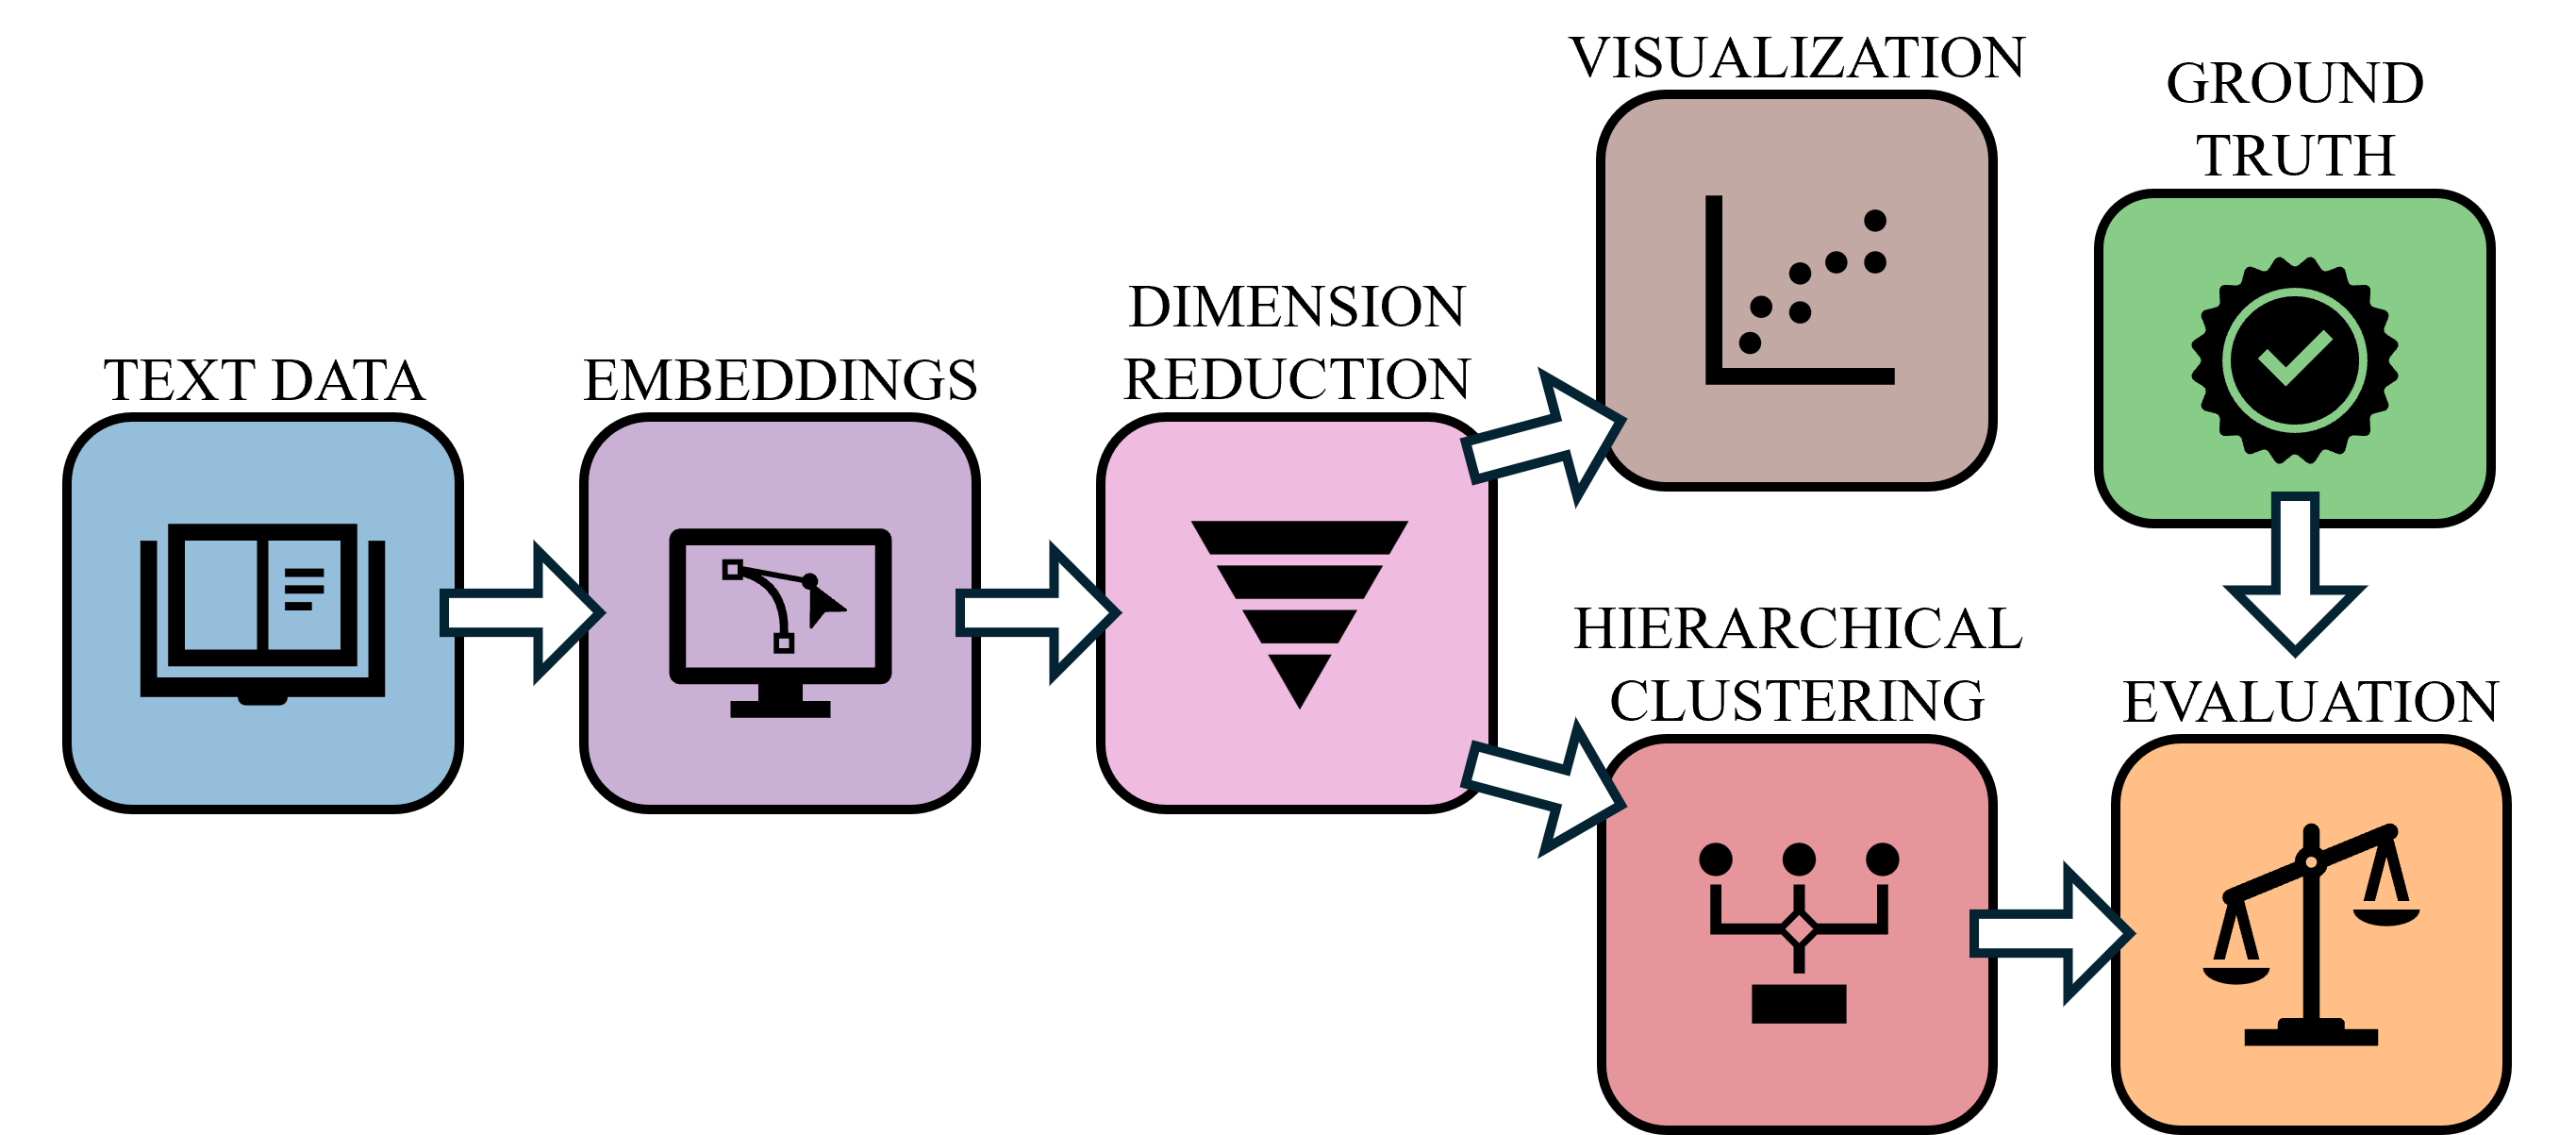
\includegraphics[width=1\linewidth]{workflow.png}
    \caption{The workflow used for studying PHATE for visualization and hierarchical clustering of text}
    \label{fig:workflow}
\end{figure}

We show that a multiscale variant of PHATE \cite{kuchroo2022multiscale} is competitive with popular hierarchical clustering pipelines that combine UMAP or PCA with agglomerative clustering or HDBSCAN. We further apply this method to a newly curated dataset of environmental policy narratives from US stakeholders, finding that PHATE yields more informative visualizations than standard approaches. These results open the door to new modes of textual analysis and motivate further extensions of PHATE beyond biological domains.

\section{Background}
Data analysts, journalists \cite{young2018makes}, and social scientists \cite{brugnone2024ought, benkler2024recognizing, friedman2024bottom} increasingly seek to turn vast amounts of unstructured text into actionable insights by curating its semantic content. Examples of such corpora include social media discussions, scientific articles, and government white papers. While text summaries can highlight key information like sentiment and argumentation by tying together salient features with narrative flow, modern NLP tools like BERTopic \cite{grootendorst2022bertopic} allow for deeper information extraction and summarization through unsupervised pipelines designed for classification and visualization. The expressiveness of these NLP tools is increasing due to high-quality vector embeddings produced by large language models (LLMs).

Text embeddings are high-dimensional, numerical representations of language, often produced as a byproduct of neural network training. These $d$-dimensional unit vectors live on the $(d-1)$-sphere, where inner products (i.e., cosine similarity) quantify semantic similarity. Recent work \cite{park2024the} suggests that the geometry of text embeddings encodes rich semantic structure, extending beyond cosine similarity.

Dimensionality reduction techniques like Principal Component Analysis (PCA) and Uniform Manifold Approximation and Projection (UMAP) \cite{mcinnes2018umap} aim to capture semantic nuance by leveraging the (linear or nonlinear) manifold structure of embeddings. The manifold hypothesis—asserting that although data lies in a high-dimensional ambient space, it approximately resides on a low-dimensional submanifold \cite{narayanan2010sample}—is central to these approaches. This hypothesis helps circumvent the curse of dimensionality and enables statistical techniques such as kernel density estimation in high dimensions. As demonstrated in, e.g., \citet{coifman2006diffusion}, \citet{moon2019visualizing}, \citet{haghverdi2015diffusion}, and others it is possible to invoke the manifold hypothesis to leverage data geometry and improve upon methods like PCA and t-SNE. Can this perspective be applied to unfurl the expressive geometry hidden within LLM text embeddings? 

\subsection{PHATE}
The manifold hypothesis has inspired significant advances in the analysis of single-cell RNA sequencing (scRNA-seq) data \cite{moon2019visualizing}, which consists of tens-of-thousands of gene expression measurements from thousands of cells. These data exhibit characteristics that include gene dropout and batch effects, which complicate statistical analysis. Moreover, subsamples of cells often follow trajectories along developmental pathways in gene expression space \cite{moon2019visualizing}. These properties led to the development of PHATE, a manifold learning technique that leverages both local and global data geometry to produce low-dimensional embeddings that preserve this structure.

Large-scale textual datasets share many structural characteristics with scRNA-seq data. The uneven expression of social and cultural signals means that important ideas may appear only in small subsets of documents—analogous to dropout. Batch effects also arise in textual data due to differing media preferences (e.g., Bluesky vs. Truth Social) and context dependency, complicating comparison across sources. In addition, narrative arcs in text resemble biological trajectories and may be recoverable through embedding methods. These parallels suggest that PHATE is a promising tool for text analysis. However, this potential has not been systematically evaluated. Here, we present a qualitative analysis of PHATE as a visualization tool and a quantitative assessment of its performance in hierarchical clustering of text.

\subsection{Hierarchical clustering}
A multiscale version of PHATE utilizing diffusion condensation \cite{brugnone2019coarse} has shown promise for identifying hierarchical structure in biological data \cite{kuchroo2022multiscale}. Similar to biology, textual data too contain latent hierarchies that are often overlooked when analyzed at a single level of granularity. Semantic content can be more richly understood by recognizing these hierarchical relationships.

Manually curated resources like WordNet capture lexical hierarchies using synsets. However, unstructured textual corpora typically lack metadata to indicate such relationships. Connections between broad concepts (e.g., “the economy”) and finer-grained topics (e.g., “employment,” “inflation”) must be inferred from the data, which necessitates either laborious and subjective manual labeling or the application of unsupervised machine learning methods.

Early automated approaches inferred hierarchies by analyzing term co-occurrence statistics \cite{sanderson1999deriving}. Modern embeddings have surpassed these methods, enabling more nuanced clustering. The standard pipeline for hierarchical clustering of text involves: (1) embedding the documents, (2) reducing the dimensionality, and (3) applying clustering algorithms at multiple levels of granularity. PCA and UMAP are frequently used for dimensionality reduction, followed by agglomerative clustering or HDBSCAN. Such methods have enabled topic modeling and sentiment analysis, but there may be an opportunity to improve upon them with more expressive coordinates.

In this paper we evaluate PHATE’s ability to generalize to text by examining how well it: (1) recovers known concept hierarchies when coupled with hierarchical clustering, and (2) visualizes semantic relationships among documents. We compare PHATE’s performance to that of PCA, UMAP, and t-SNE (t-distributed Stochastic Neighbor Embedding) across a range of parameter settings and evaluate their ability to produce more informative visualizations and to recover ground-truth hierarchies when coupled with hierarchical clustering.


\section{Methods}
Dimensionality reduction techniques such as PCA, UMAP \cite{mcinnes2018umap}, and t-SNE \cite{van2008visualizing} are widely used for visualizing high-dimensional data. While PCA preserves global linear structure, nonlinear methods like UMAP and t-SNE focus on local neighborhood preservation, often at the expense of global relationships.

PHATE \cite{moon2019visualizing} was introduced to better capture both local and global structure through diffusion geometry, and has been successfully applied in biological and scientific data analysis. However, its application to large-scale textual data remains less explored.

In hierarchical clustering evaluation, traditional metrics such as ARI and AMI do not capture structural relationships between clusters. Prior work has introduced structure-aware metrics such as LCA-F1 \cite{kosmopoulos2015} and dendrogram purity \cite{heller2005bayesian}, which evaluate agreement between hierarchical structures. These metrics have been shown to provide more meaningful evaluation for hierarchical classification tasks \cite{kosmopoulos2015}

\subsection{Dimensionality reduction \& visualization}
To evaluate its utility for text, we compare PHATE visualizations against those from PCA, UMAP, and t-SNE.
\begin{description}
    \item[PCA] reduces dimensionality by projecting data onto the leading eigenvectors of the covariance matrix, preserving global linear structure.
    \item[UMAP] uses a weighted k-nearest neighbor (kNN) graph and a nonlinear embedding based on force-directed layout \cite{mcinnes2018umap}.
    \item[t-SNE] forms a probability distribution over pairwise dissimilarities and embeds points such that the KL divergence between the original and embedded distributions is minimized \cite{van2008visualizing}
    \item[PHATE] also constructs a weighted kNN graph, row-normalizes its adjacency matrix to a Markov operator, amplifies global structure by powering the operator, computes information distances using row-wise log-transforms, and applies metric multidimensional scaling to derive low-dimensional coordinates \cite{moon2019visualizing}.
    \item[PaCMAP] (Pairwise Controlled Manifold Approximation) balances preservation of both local and global structure by explicitly controlling pairwise relationships during embedding optimization \cite{wang2021pacmap}.
    \item[TriMAP] emphasizes preservation of global structure by optimizing triplet relationships between points, ensuring that relative distances are maintained in the low-dimensional embeddingTriMAP \cite{trimap}.
\end{description}
\textit{Qualitative comparisons} are made using datasets with ground-truth metadata. Evaluation criteria include cluster coherence, separation of known categories, and preservation of trajectories or arcs in embedding space.
\subsection{Text Embeddings}

We generate dense semantic embeddings using two models: all-MiniLM-L6-v2 and Qwen3-Embedding-0.6B. Each document is converted into a high-dimensional vector representation capturing semantic meaning.

For Qwen embeddings, text inputs are tokenized and transformed into 1024-dimensional vectors. Mean pooling is applied to obtain a single representation per document, followed by L2 normalization to ensure consistent similarity comparisons.
\subsection{Hierarchical clustering}

To assess PHATE in clustering, we:
\begin{enumerate}
\item Generate datasets with known hierarchical structure (see "Datasets").
\item Embed the data using pre-trained language models, including \texttt{all-MiniLM-L6-v2} and \texttt{Qwen3-Embedding-0.6B}.
\item Apply PCA, UMAP, PHATE, PaCMAP, and TriMAP for dimensionality reduction.
\item Cluster with agglomerative clustering (Ward's method), HDBSCAN, Diffusion Condensation, and HERCULES.
\end{enumerate}

\paragraph{Clustering Methods.}
We evaluate multiple clustering approaches on the reduced embeddings.

Agglomerative clustering constructs a hierarchical tree using Ward linkage, enabling direct evaluation of hierarchical structure.

HDBSCAN is a density-based clustering method that identifies clusters of varying density while labeling noise points automatically.

Diffusion Condensation builds hierarchical structure through an iterative diffusion process, progressively merging points based on similarity.

HERCULES is an LLM-based hierarchical clustering framework that constructs topic hierarchies using semantic reasoning and recursive partitioning.
These methods were selected to compare hierarchical and density-based clustering approaches under a unified embedding and reduction pipeline.
\subsection{Experimental Pipeline}

We apply dimensionality reduction methods, including PCA, UMAP, PHATE, PaCMAP, and TriMAP, to obtain low-dimensional representations.
Clustering is performed on each reduced representation using Agglomerative Clustering, HDBSCAN, Diffusion Condensation, and HERCULES. All methods operate on identical precomputed embeddings to ensure that performance differences arise solely from the dimensionality reduction and clustering methods.
\paragraph{Evaluation Metrics.}
We evaluate clustering performance using AMI, ARI, Fowlkes–Mallows (FM), and Rand Index. 
For dimensionality reduction, we use trustworthiness, continuity, Shepard diagrams, Spearman correlation, and DEMaP.
\subsection{Datasets}
To assess the visual quality of PHATE embeddings, public comments from the Environmental Protection Agency (EPA) were sourced from the Federal Register via Regulations.gov as part of a related project studying public perceptions and preferences as related to environmental policy. The data was collected from an open source initiative called Mirrulations\footnote{https://registry.opendata.aws/mirrulations/}, which mirrors this public data through an Amazon Web Services S3 bucket. Once the data was gathered, the text was cleaned by removing HTML tags, special characters, URLs, stop words, and excessively short entries, focusing only on comments submitted after the year 2000. To handle long comments and improve compatibility with transformer models, a head-tail truncation strategy \cite{sun2019fine} was used to preserve meaningful content from the beginning and end of each comment. The cleaned data was embedded using the sentence-transformers model all-\texttt{MiniLM-L6-v2}. 
To evaluate clustering quality, we required hierarchical text datasets with known ground truth. As no available datasets met our application needs, we generated synthetic datasets using an LLM. We curated two thematic seeds—\textit{Energy, Ecosystems, and Humans} and \textit{Offshore Energy Impacts on Fisheries}—to span a range from general to domain-specific topics related to our parallel applied research in social-ecological systems modeling. From each seed, we recursively generated hierarchical structures of varying depth and breadth, simulating both shallow and deeply nested trees.

To mimic the irregularities of real-world ontologies, we varied the number of children per node at random. A labeling heuristic propagated parent labels to children while excluding the parents themselves from deeper levels, reflecting semantic containment without conflating hierarchical roles. To further simulate real-world messiness, we injected structural noise in the form of concepts from overlapping subtopics and ambiguous nodes. 
% These elements challenged models to infer latent structure and semantic grouping.
The resulting datasets were used for both quantitative benchmarking and qualitative analysis of PHATE’s capacity to capture semantic and hierarchical organization in text.

To assess performance across diverse hierarchical domains, we applied our methods to benchmark datasets with known hierarchies, including Web of Science paper keywords \cite{kowsari2017HDLTex}, Wikipedia article categories \cite{brummer2016dbpedia, NIPS2015_250cf8b5, yang2019xlnet}, Amazon product reviews \cite{yury_kashnitsky_2020}, arXiv \cite{arxiv_kaggle}, with hierarchical labels derived from the arXiv category taxonomy \cite{arxiv_taxonomy}. The data was accessed via a publicly available Kaggle mirror. We also use the RCV1 dataset \cite{lewis2004rcv1}.

\begin{table}[ht]
    \centering
    \caption{Number of datapoints in each dataset.}
    \begin{tabular}{l l l r}
    \hline
    \textbf{Category} & \textbf{Topic} & \textbf{Depth} & \textbf{N} \\
    \hline
    \multirow{4}{*}{Generated} 
     & \multirow{2}{*}{Ecosystems} & Deep & 19{,}469 \\
     &  & Shallow & 4{,}848 \\
     & \multirow{2}{*}{Fisheries} & Deep & 19{,}806 \\
     &  & Shallow & 6{,}708 \\
    \hline
    \multirow{5}{*}{Benchmark}
     & \multicolumn{2}{l}{WoS} & 46{,}985 \\
     & \multicolumn{2}{l}{DBpedia} & 60{,}794 \\
     & \multicolumn{2}{l}{Amazon} & 14{,}824 \\
     & \multicolumn{2}{l}{arXiv} & 30{,}000 \\
     & \multicolumn{2}{l}{RCV1} & 1{,}628 \\
    \hline
    \end{tabular}
    \label{tab:dataset_counts}
    \end{table}

\section{Results}
\subsection{Visualization}
\begin{figure*}
    \centering
    \includegraphics[width=1\textwidth]{all_embeddings_subplot_copy.png}
    \caption{Visualizations of datasets with known hierarchical structure; (d) and (s) correspond to generated deep and shallow hierarchies, respectively. Multiclass noise in generated data is depicted in gray.}
    \label{fig:panel-fig}
\end{figure*}
Visualizations of text embeddings colored by top-level categories appear in Figure \ref{fig:panel-fig}. The generated hierarchies with 25\% noise are visualized. PHATE and PCA are better able to separate the noise class as compared with t-SNE and UMAP, but PHATE better preserves noise semantics by its centralized location, indicating a relation with multiple classes. PCA and t-SNE plots are globally quite similar, but t-SNE provides more class discriminability. PHATE, by contrast, displays top-level categories as extremal points of the embedding and provides cleaner class separation than PCA and t-SNE. UMAP collapses most of the information onto a single dimension in some cases and in others bears similarity to PHATE although compressing points and, in some cases, shattering the global structure. Additional visualizations with default parameter settings for UMAP and PHATE are provided in the appendices in Figure \ref{fig:default-visuals}.

The trajectory of topics and themes in the visualizations can be analyzed in several different ways. We visualize how the sub-themes within the Ecosystems data transition between the two themes of "Economic Impact Metrics" and "Social Conflict Intensity" (Figure \ref{fig:ecosystems-trajectory}). Similarly with the Fisheries data, we use the specific concepts to determine how some of the sub-themes mapped between the categories of "Offshore Energy Infrastructure Development," "Marine Environmental Quality," and "Fish Population Metrics" (Figure \ref{fig:fisheries-trajectory}). We, furthermore, curate semantic trajectories in the Web of Science embedding on the basis of keywords associated to each data point as provided in the dataset (Figure \ref{fig:WoS-trajectory}). Lastly, we use the information at the docket level for the EPA data to determine thematic changes over space (Figure \ref{fig:epa-trajectory}). 

\begin{figure*}
    \centering 
\begin{subfigure}{0.48\textwidth}
    \centering
    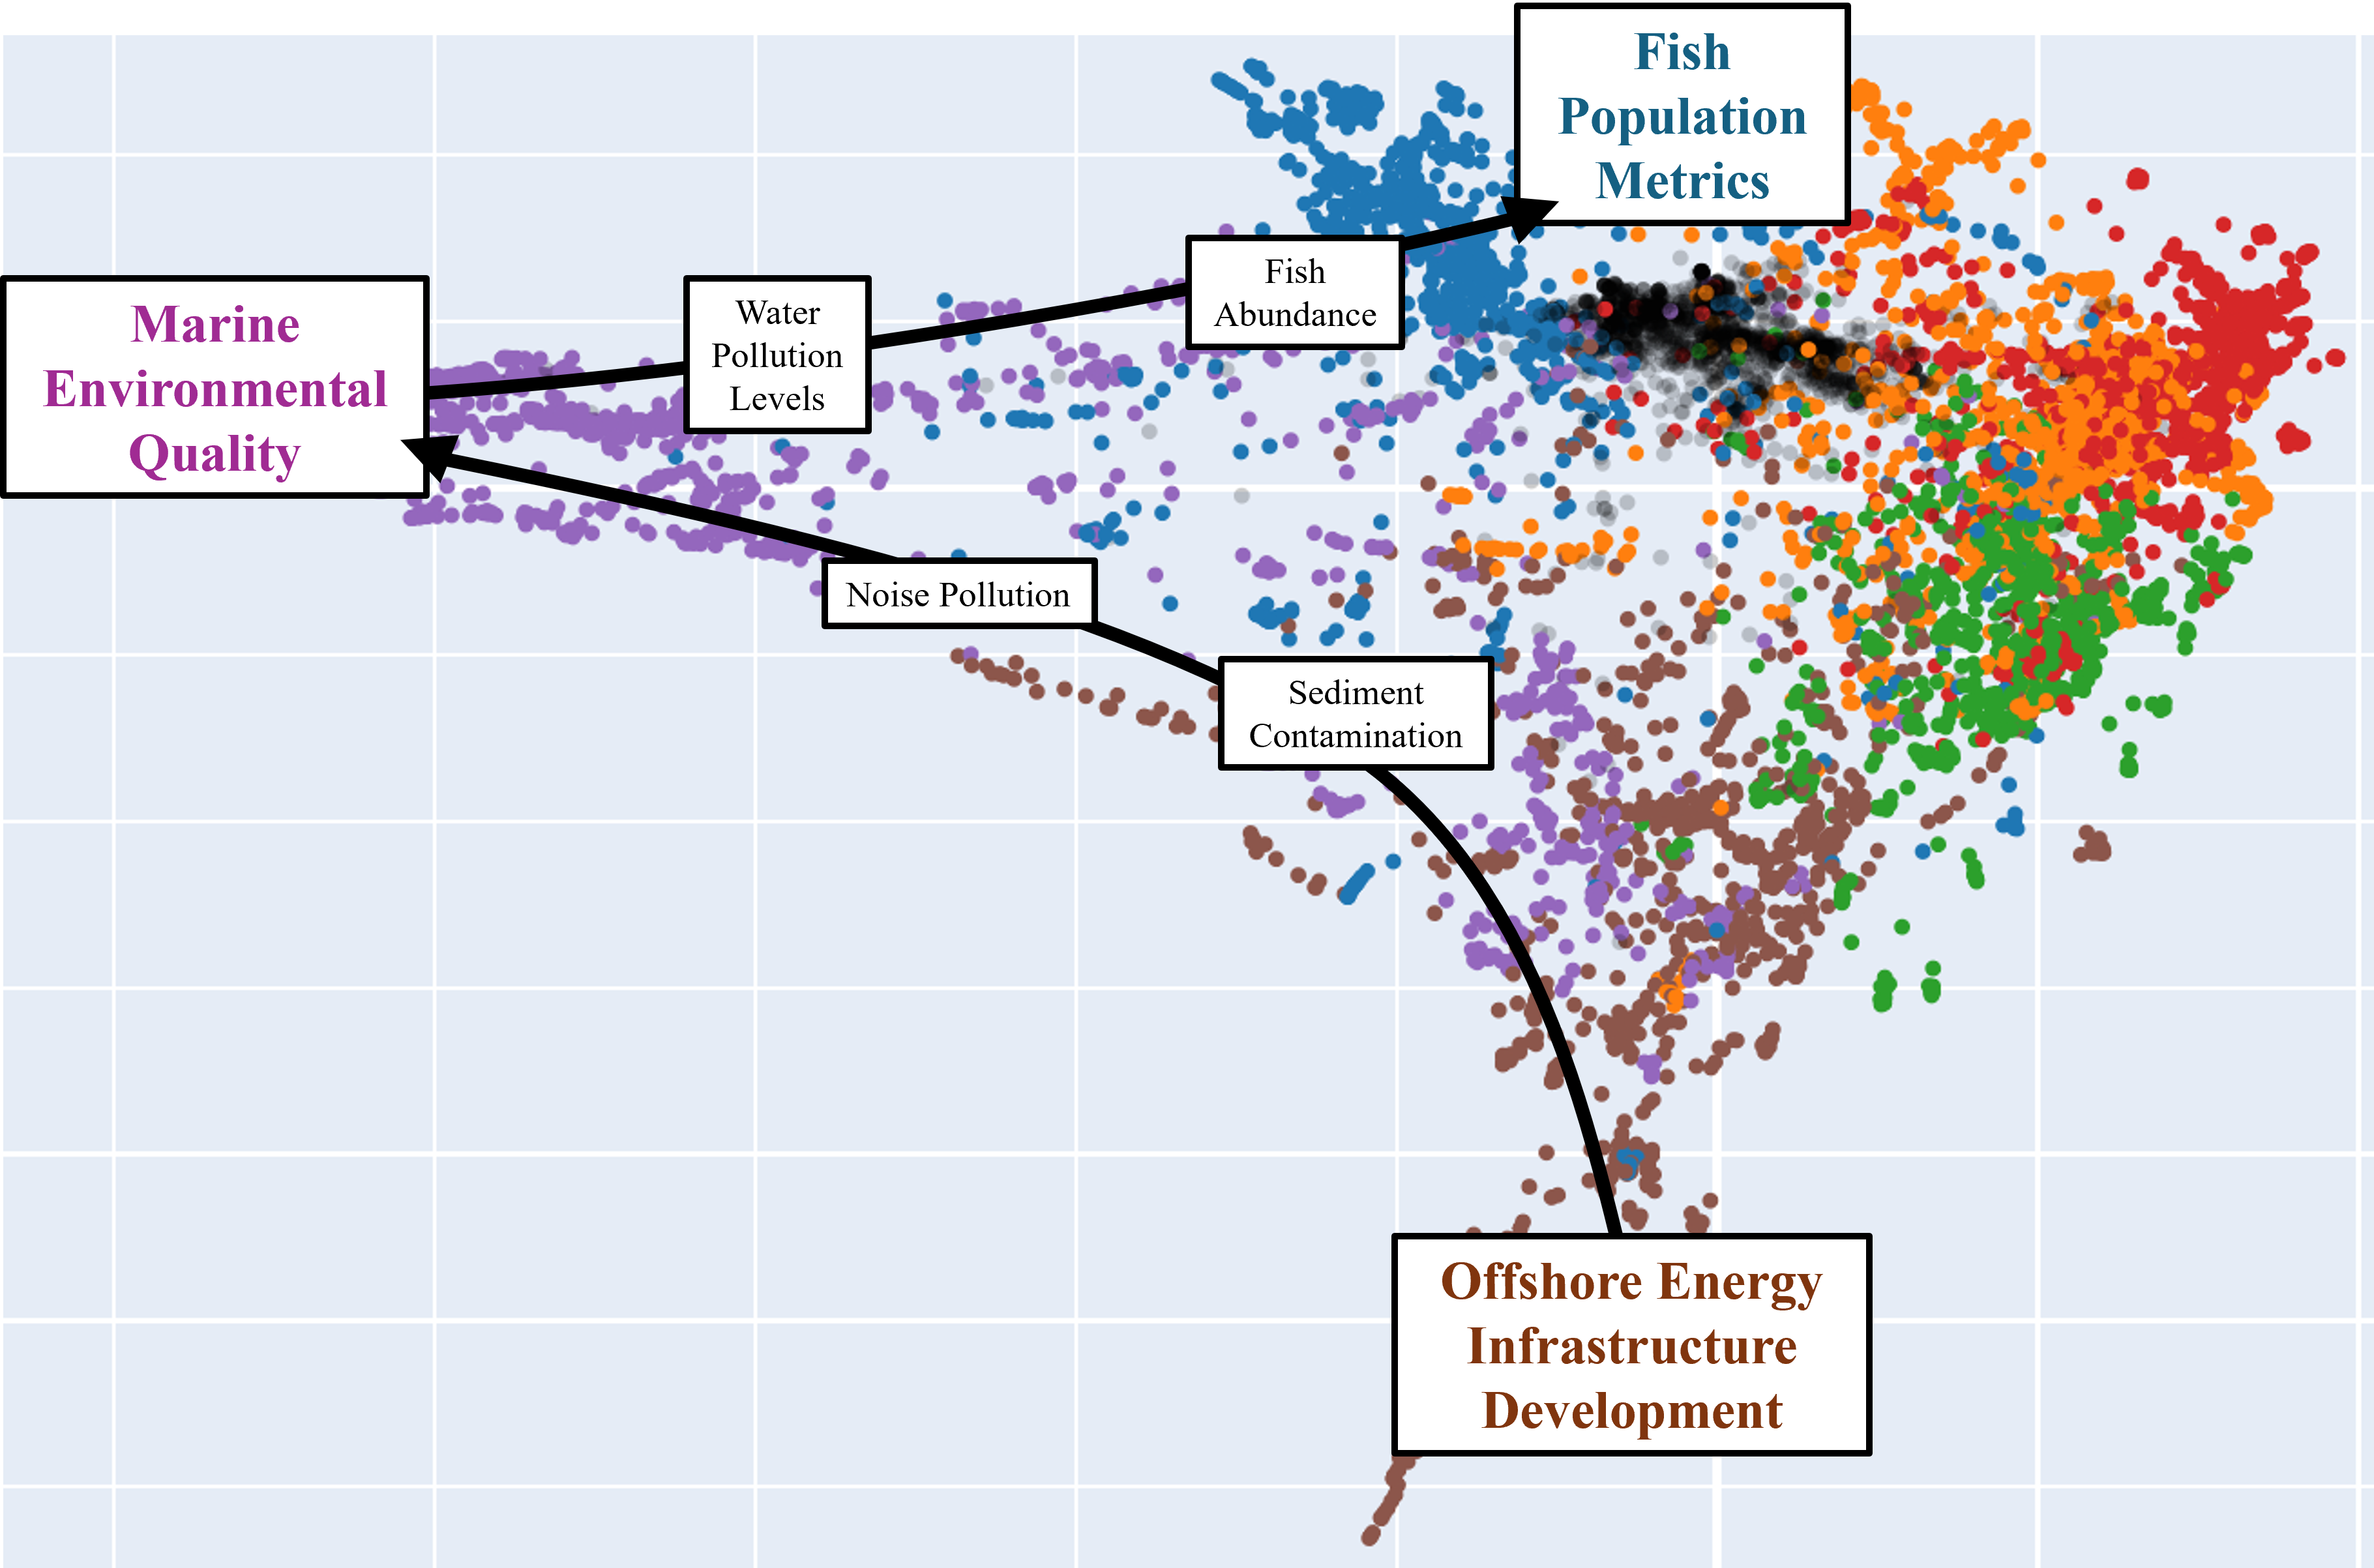
\includegraphics[width=\linewidth]{fisheries_trajectory.png}
    \caption{Trajectories in deep fisheries hierarchy}
    \label{fig:fisheries-trajectory}
\end{subfigure}
\begin{subfigure}{0.48\textwidth}
    \centering
    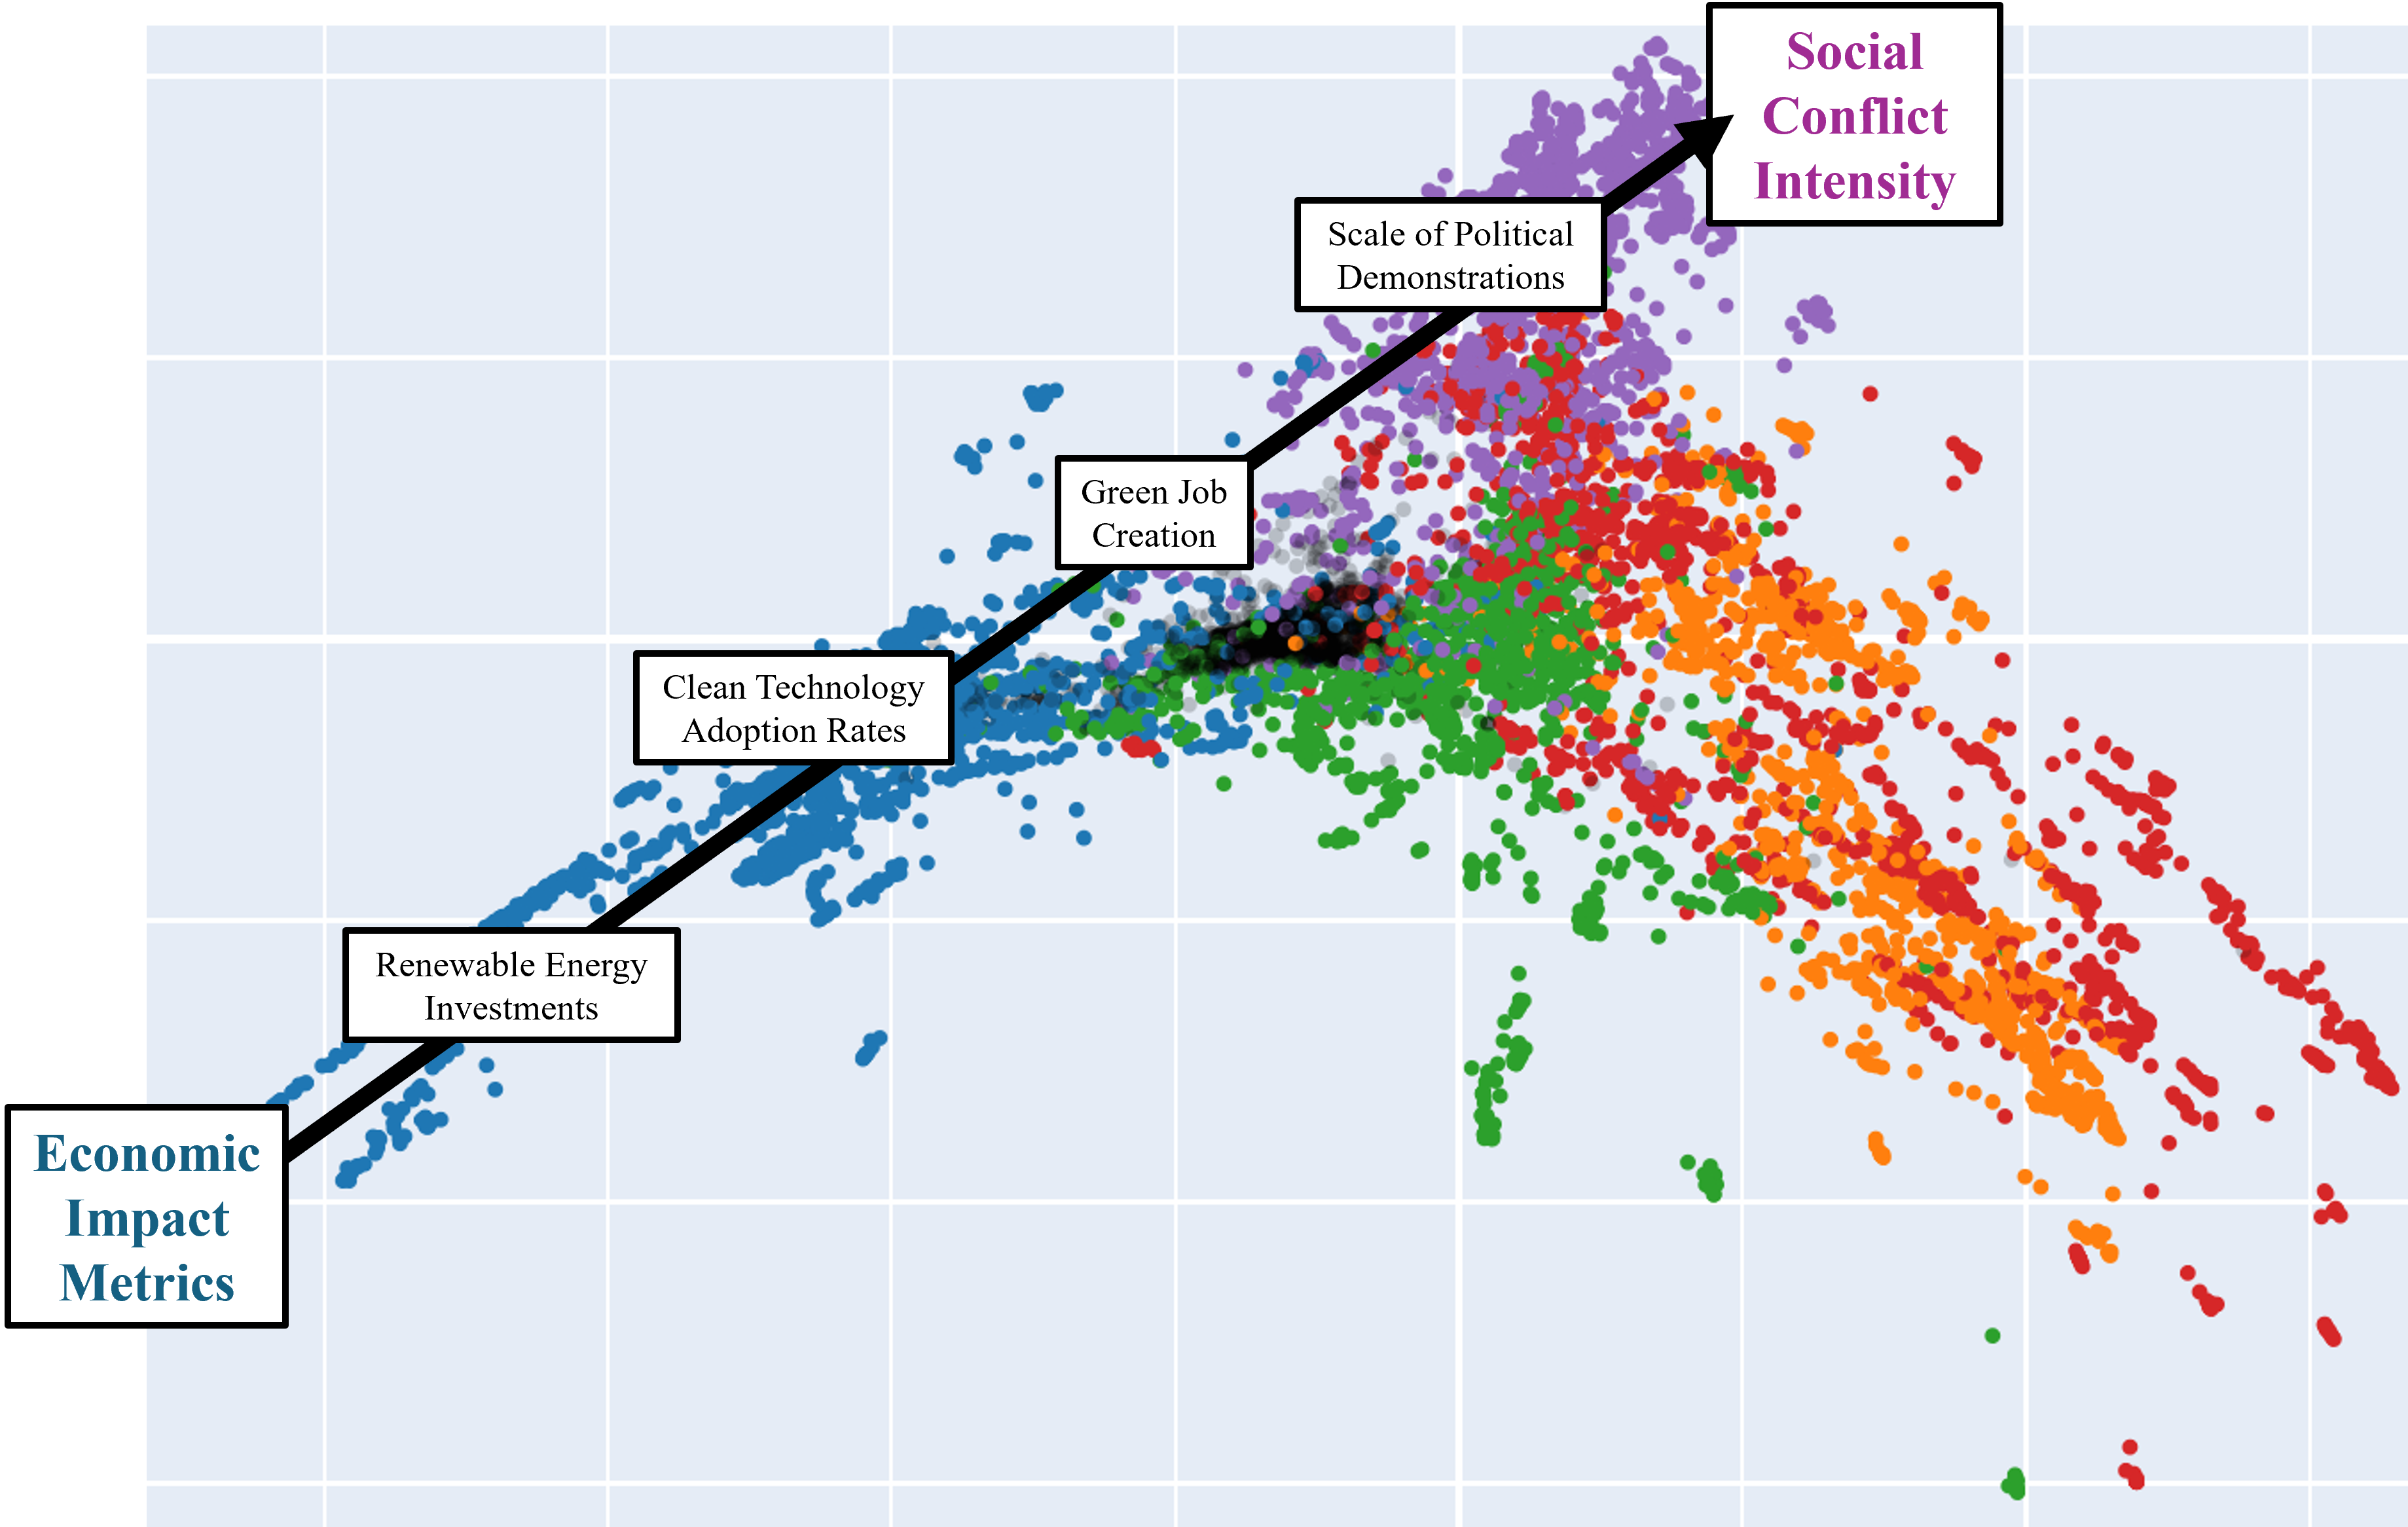
\includegraphics[width=\linewidth]{ecosystems_trajectory.png}
    \caption{Trajectories in deep ecosystems hierarchy}
    \label{fig:ecosystems-trajectory}
\end{subfigure}
\caption{"Narrative arc" trajectories in PHATE embedding space}
\label{fig:hierachy_trajectories}
\end{figure*}

\begin{figure*}
    \centering
    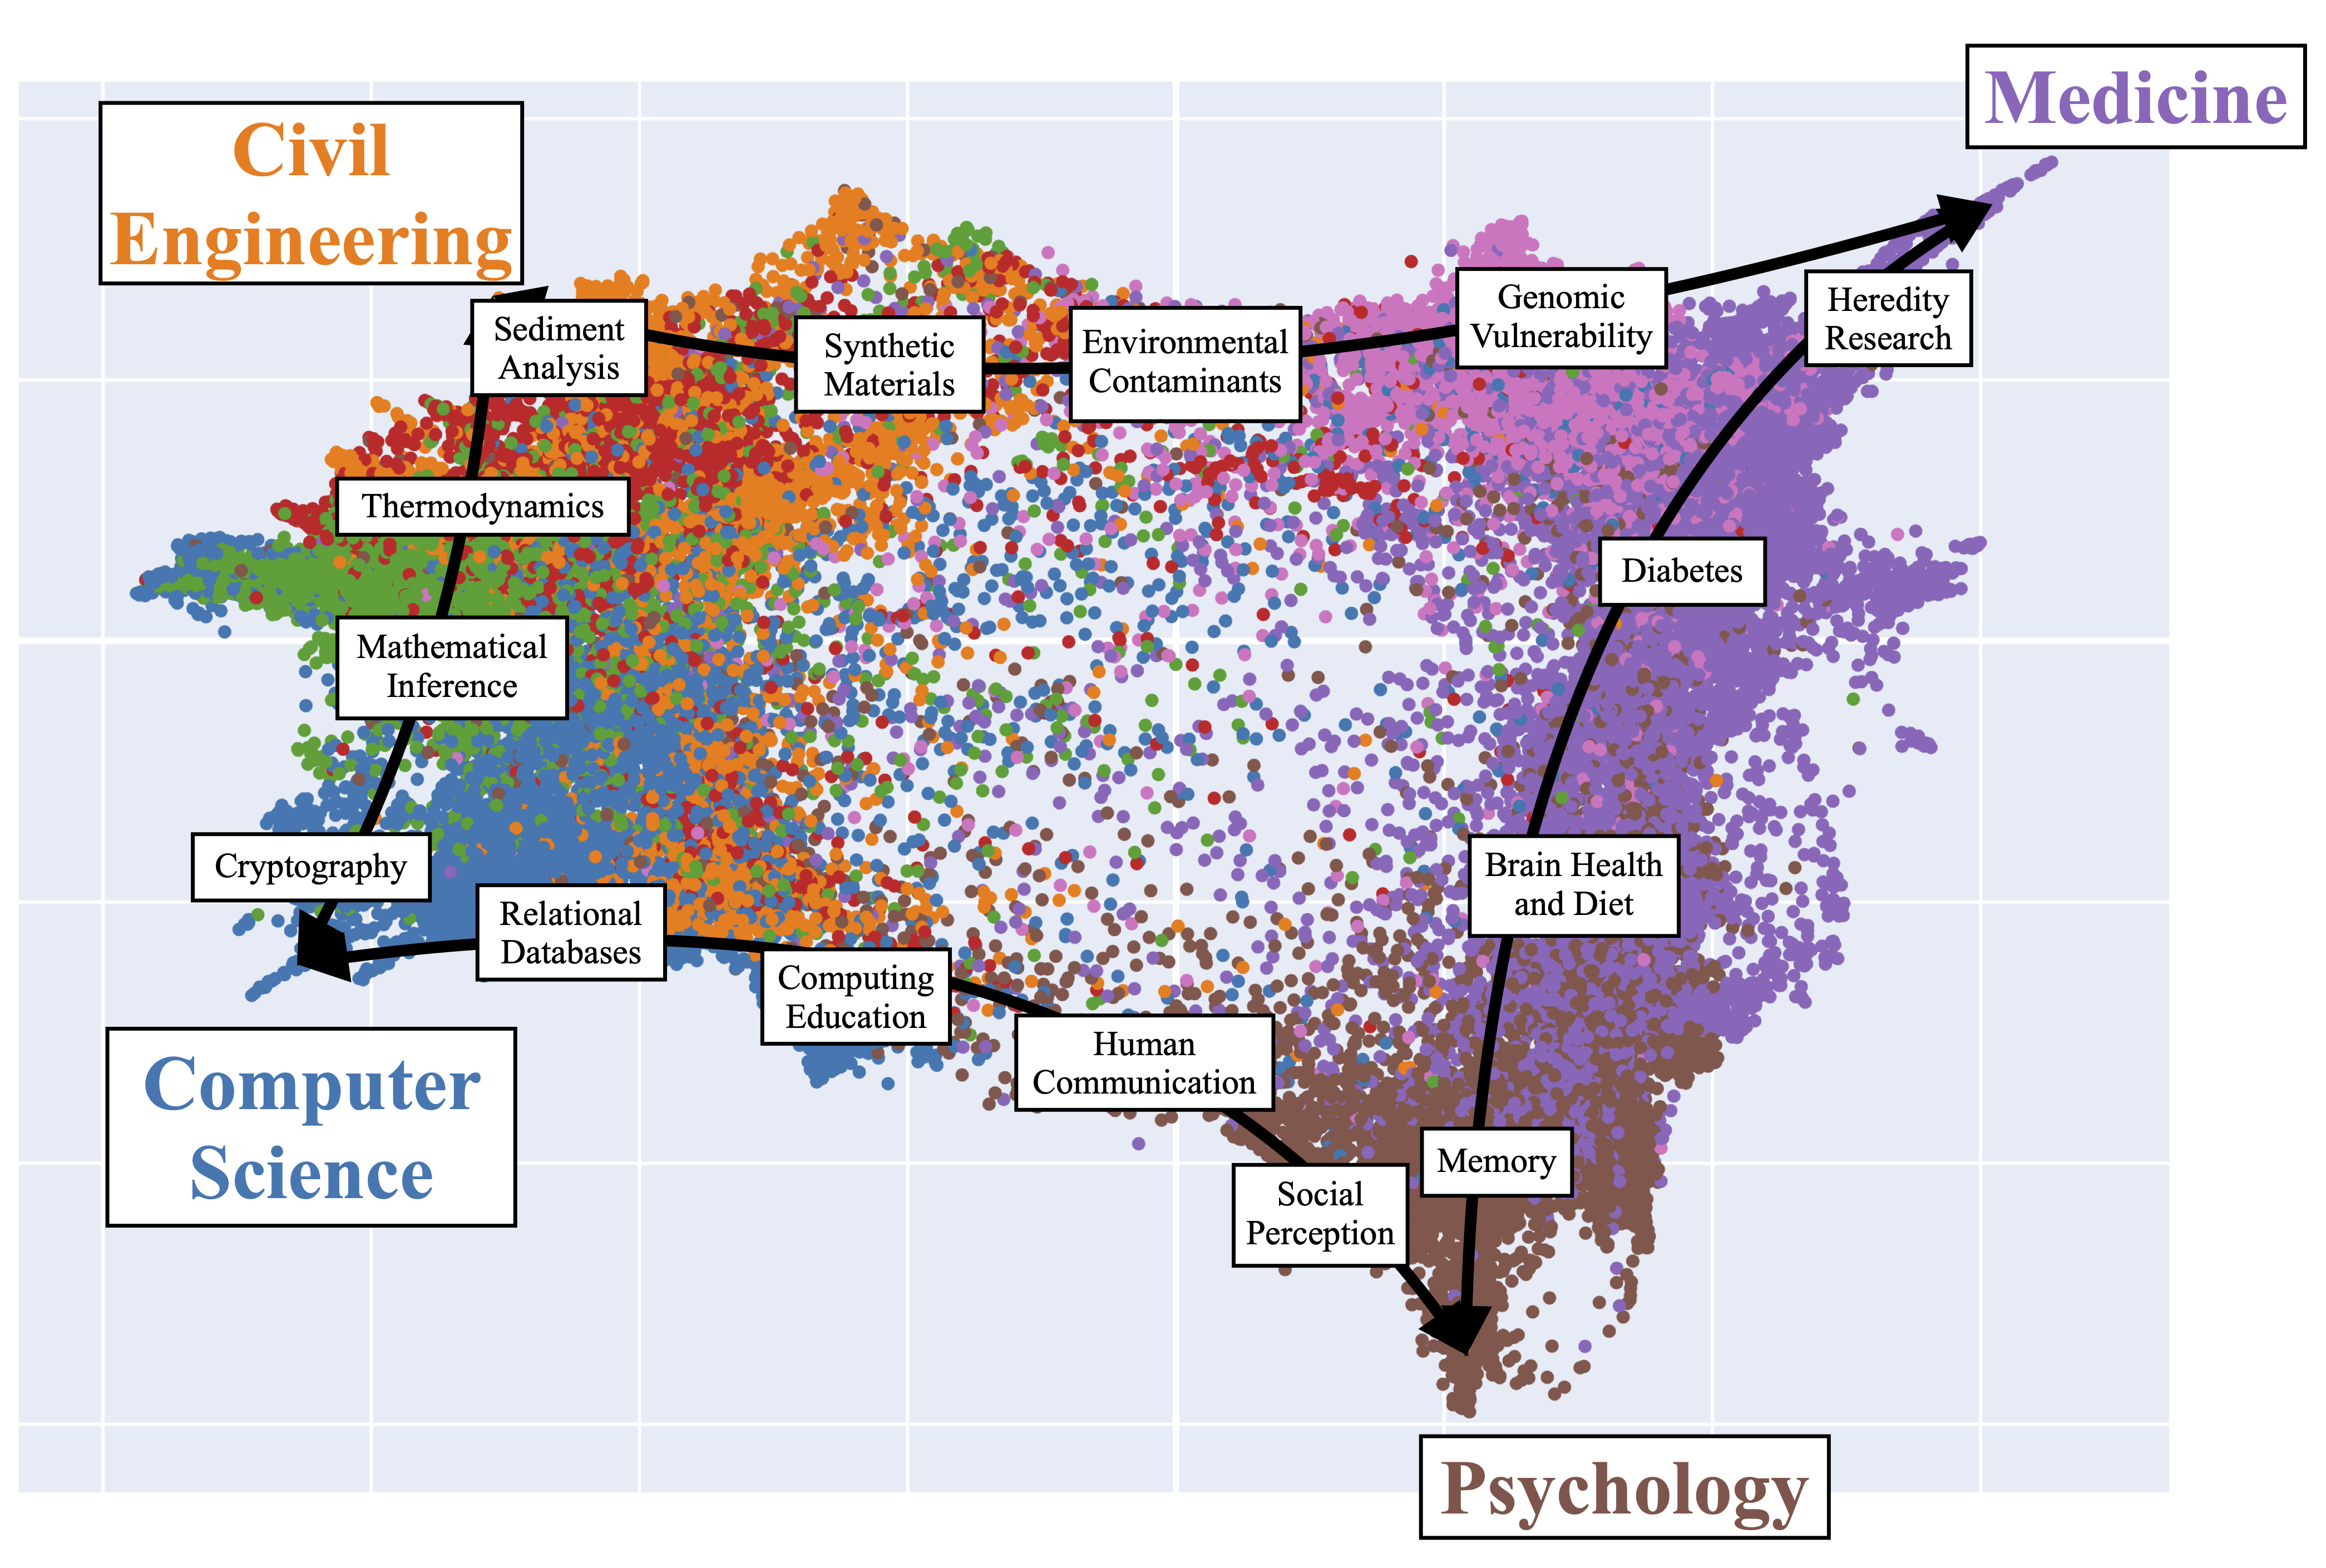
\includegraphics[width=1\linewidth]{phate_WOS.png}
    \caption{"Narrative arc" trajectories in PHATE embedding space of Web of Science}
    \label{fig:WoS-trajectory}
\end{figure*}  

\begin{figure}
    \centering
    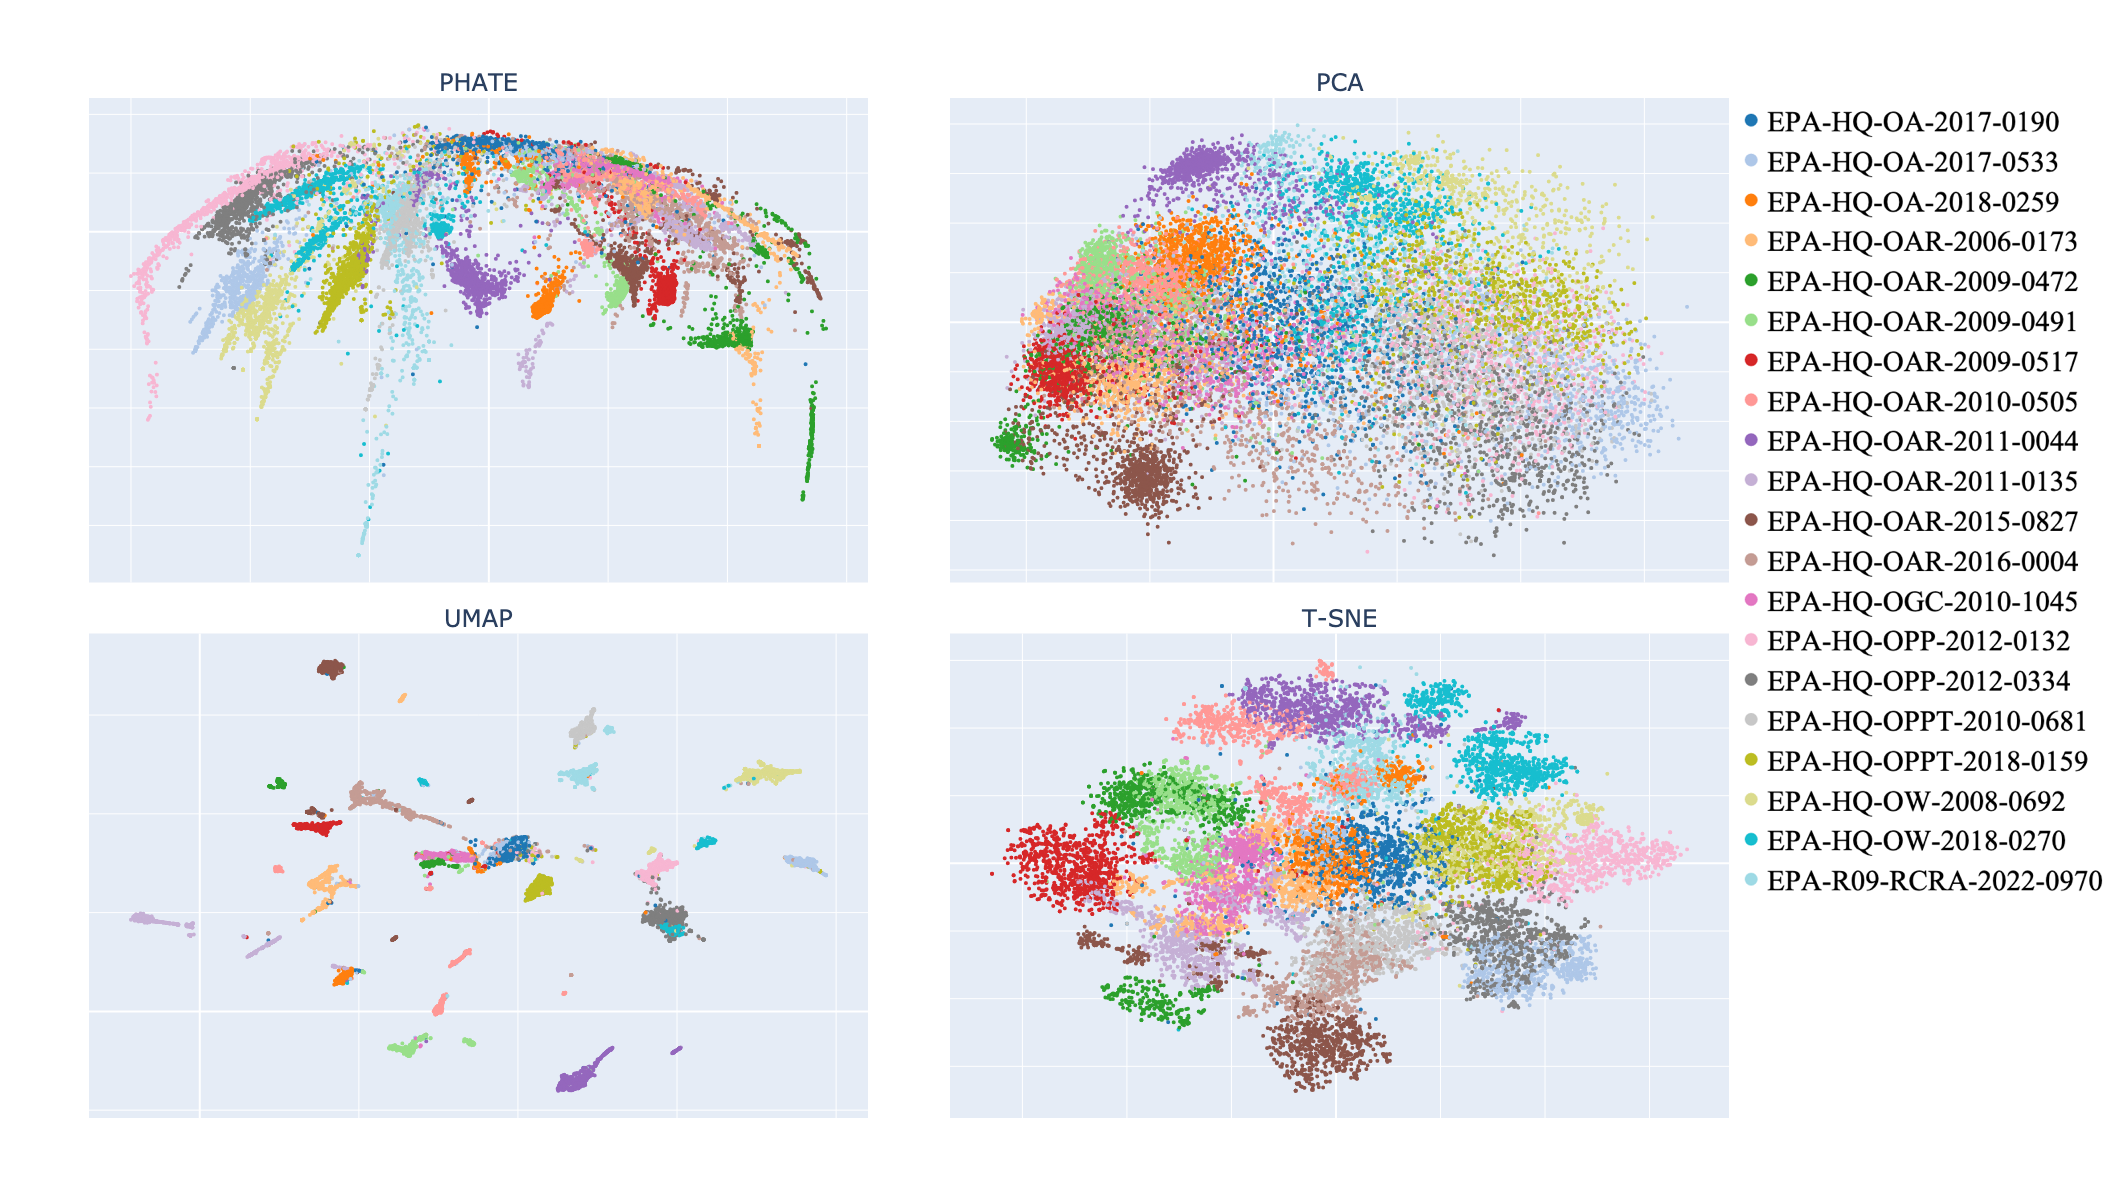
\includegraphics[width=1\linewidth]{epa_fig.png}
    \caption{Visualizations of head-tail embeddings of EPA comments colored by docket}
    \label{fig:epa-fig}
\end{figure}

\begin{figure}
    \centering
    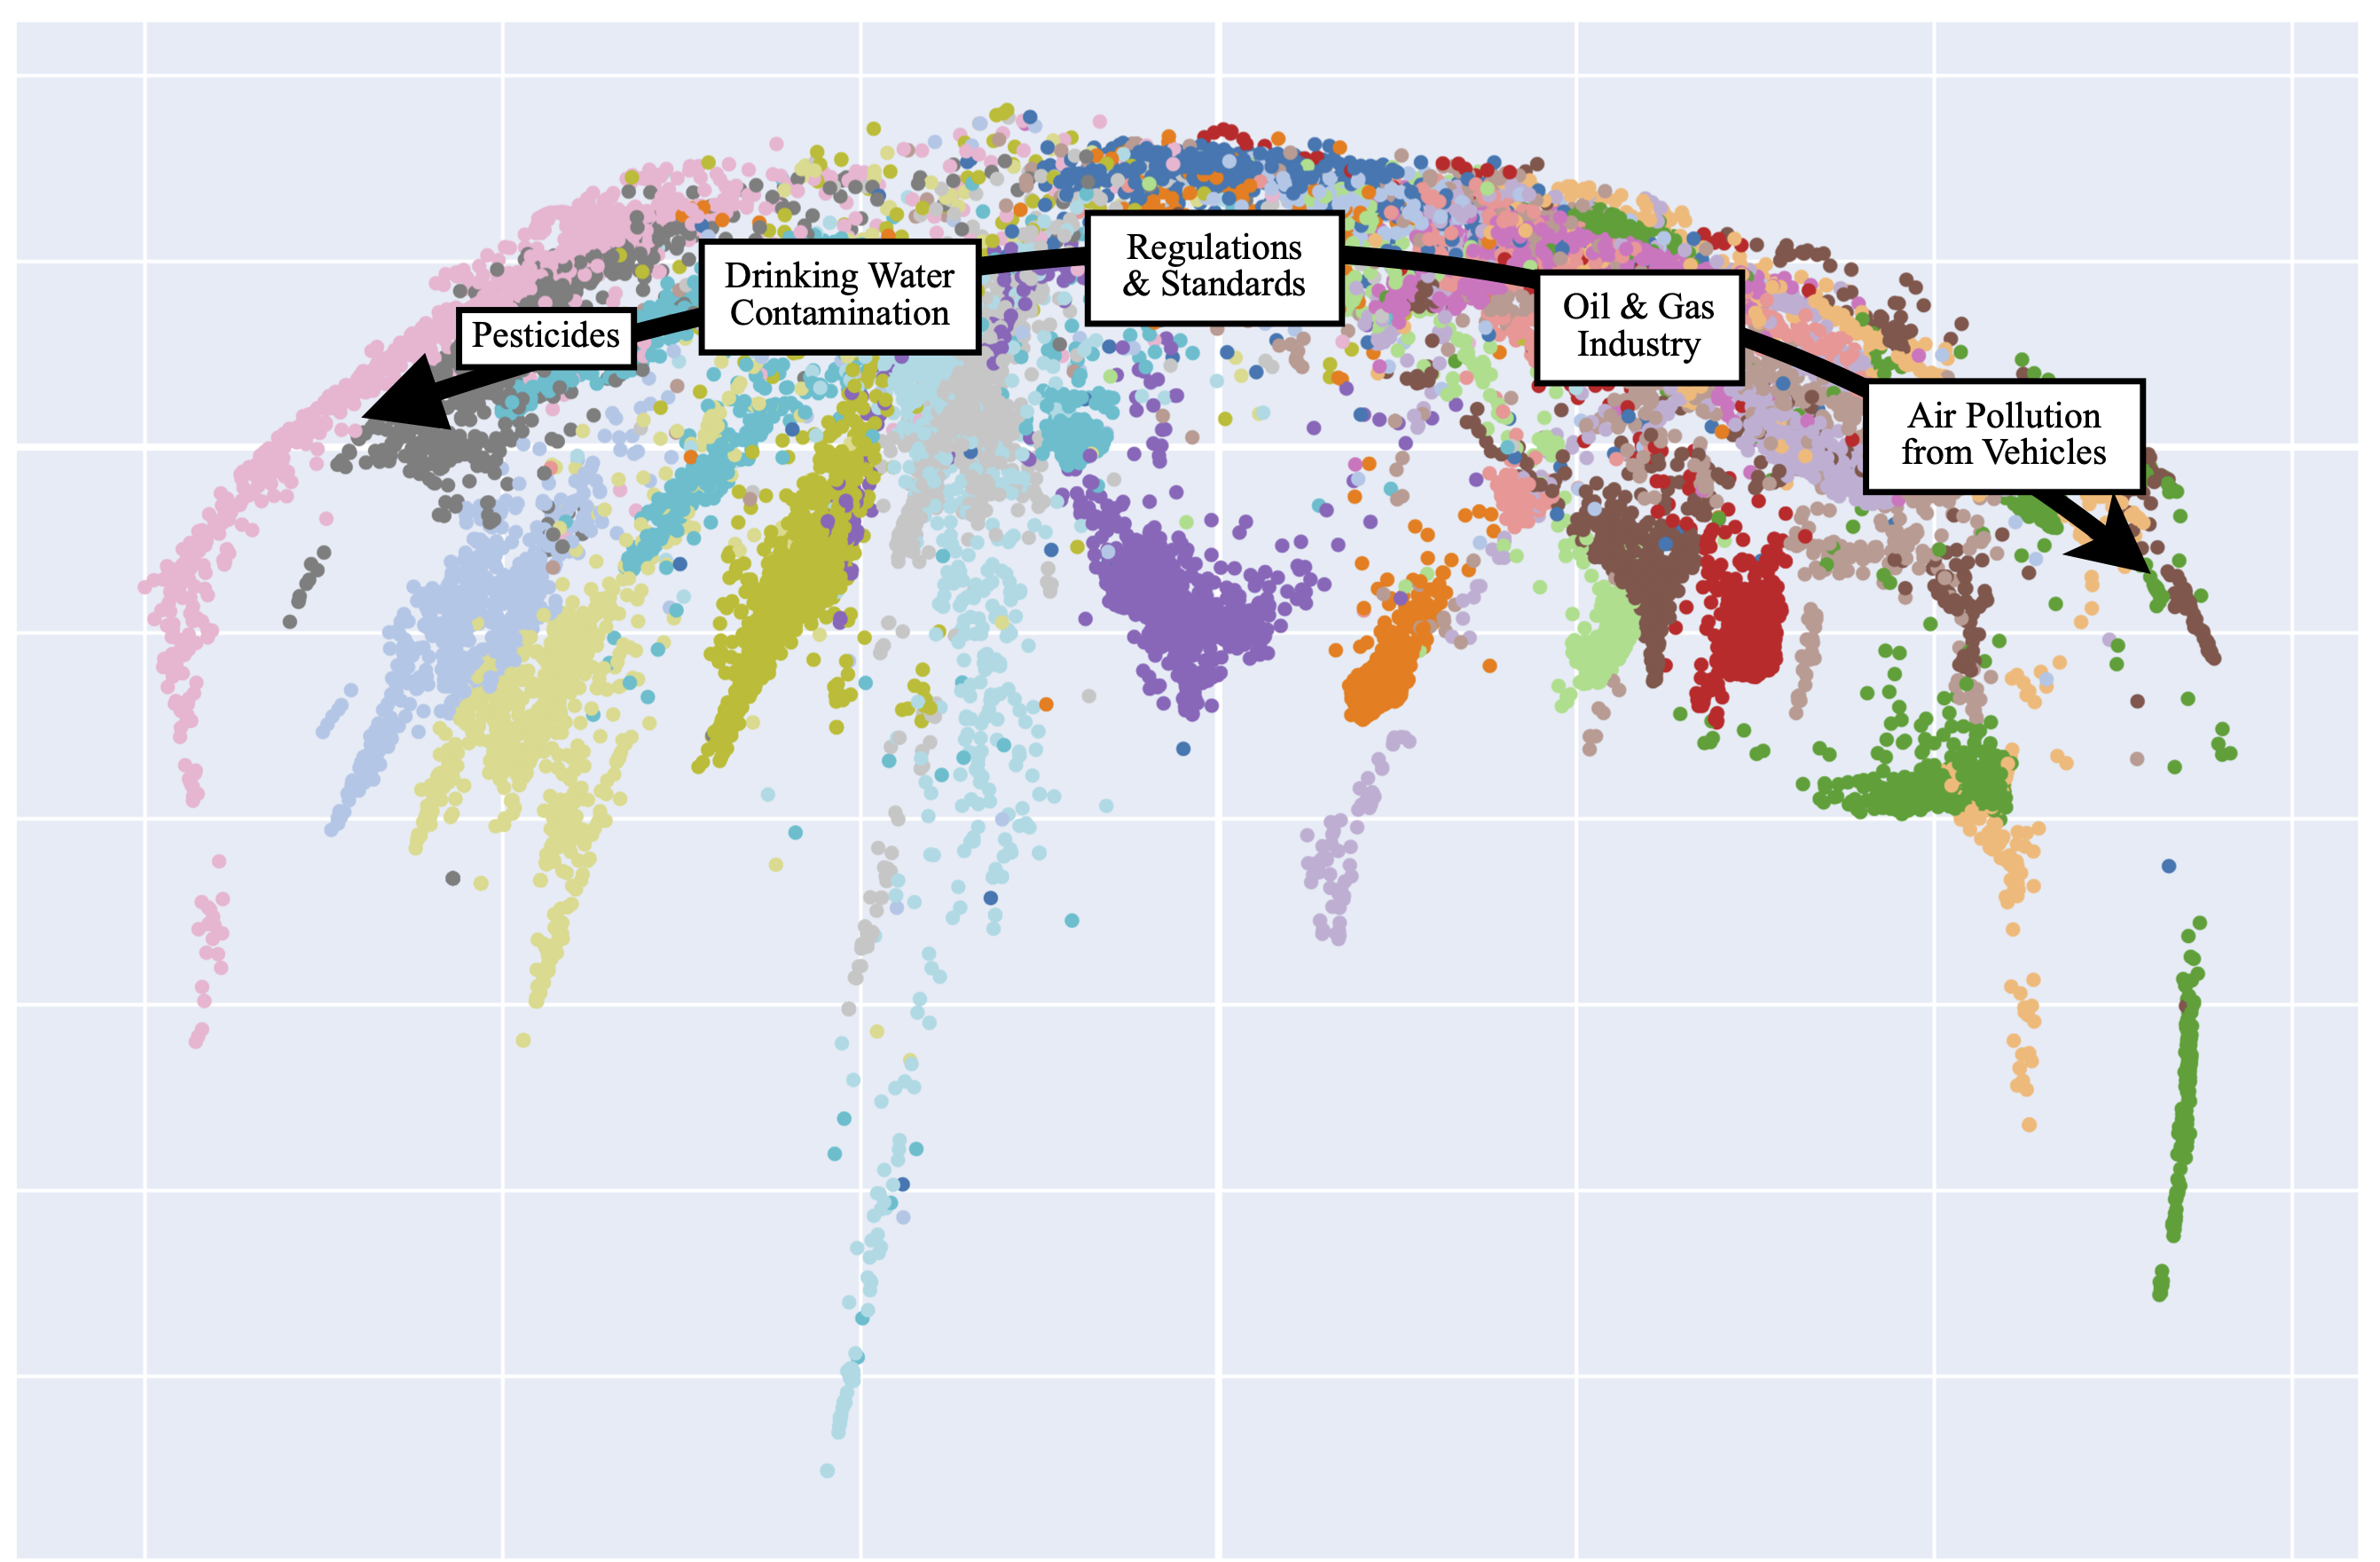
\includegraphics[width=1\linewidth]{epa_trajectory.png}
    \caption{"Narrative arc" trajectories in PHATE embedding space of EPA comments}
    \label{fig:epa-trajectory}
\end{figure}  

The visualization of PHATE compared to PCA, t-SNE and UMAP colored by the top 20 dockets is shown in Figure \ref{fig:epa-fig}. While PCA produces a dense and overlapping projection with limited visible structure, and t-SNE and UMAP highlight isolated clusters with distorted global relationships, PHATE preserves both local and global geometry using branching structures which suggest underlying transitions in comment themes across EPA dockets.
\FloatBarrier
\subsection{Dimensionality Reduction Evaluation}

As shown in Tables \ref{tab:dr_metrics} and \ref{tab:dr_synthetic}, across all datasets, including both synthetic benchmarks and real-world datasets such as arXiv and RCV1, trustworthiness and continuity values are consistently high, particularly for UMAP and PaCMAP. This indicates strong preservation of local neighborhood structure, with non-linear methods outperforming PCA and PHATE.

Shepard diagrams show deviation from the diagonal across all methods, indicating that global distances are not perfectly preserved. This suggests that dimensionality reduction introduces non-linear distortion, where distances are compressed in some regions and expanded in others.

Spearman rank correlation and DEMaP metrics further confirm moderate preservation of global structure. UMAP and PaCMAP achieve higher values across most datasets, while PCA consistently shows lower global structure preservation. These trends are consistent across datasets.

Overall, UMAP demonstrates the most consistent performance across both local and global metrics, with PaCMAP as a strong alternative, while PCA and PHATE show comparatively weaker performance.
% Real world dataset table
\begin{table*}[t]
    \centering
    \caption{Dimensionality reduction evaluation across datasets using trustworthiness, continuity, Spearman correlation, and DEMaP.}
\label{tab:dr_metrics}
    \begin{tabular}{llcccc}
    \toprule
    Dataset & Method & Trustworthiness & Continuity & Spearman & DEMaP \\
    \midrule
    RCV1 & PCA & 0.7781 & 0.8913 & 0.3965 & 0.4687 \\
    RCV1 & UMAP & 0.9563 & 0.9442 & 0.4863 & 0.6847 \\
    RCV1 & PHATE & 0.7979 & 0.9035 & 0.3725 & 0.6453 \\
    RCV1 & PaCMAP & 0.9360 & 0.9333 & 0.4218 & 0.6514 \\
    \midrule
    arXiv & PCA & 0.7606 & 0.8832 & 0.4858 & 0.4665 \\
    arXiv & UMAP & 0.9414 & 0.9290 & 0.5430 & 0.6406 \\
    arXiv & PHATE & 0.7988 & 0.8971 & 0.5796 & 0.6243 \\
    arXiv & PaCMAP & 0.9051 & 0.9274 & 0.5784 & 0.6442 \\
    \midrule
    Amazon & PCA & 0.7399 & 0.8523 & 0.3708 & 0.3605 \\
    Amazon & UMAP & 0.9164 & 0.9152 & 0.4400 & 0.5482 \\
    Amazon & PHATE & 0.7776 & 0.8833 & 0.4184 & 0.5123 \\
    Amazon & PaCMAP & 0.8645 & 0.8992 & 0.3964 & 0.4788 \\
    \midrule
    DBpedia & PCA & 0.7116 & 0.8563 & 0.3095 & 0.2374 \\
    DBpedia & UMAP & 0.9706 & 0.9371 & 0.2967 & 0.5000 \\
    DBpedia & PHATE & 0.8087 & 0.9068 & 0.2244 & 0.4385 \\
    DBpedia & PaCMAP & 0.9353 & 0.9325 & 0.2585 & 0.4501 \\
    \midrule
    WoS & PCA & 0.7866 & 0.8850 & 0.5444 & 0.5760 \\
    WoS & UMAP & 0.9504 & 0.9434 & 0.5313 & 0.7099 \\
    WoS & PHATE & 0.8505 & 0.9207 & 0.5438 & 0.7024 \\
    WoS & PaCMAP & 0.9102 & 0.9434 & 0.5289 & 0.6892 \\
    \bottomrule
    \end{tabular}
\end{table*}

% synthetic dataset (clean + noise)
\begin{table*}[t]
    \centering
    \caption{Dimensionality reduction evaluation on synthetic hierarchical datasets (depth3 and depth5) under varying noise conditions.}
    \label{tab:dr_synthetic}
    \begin{tabular}{lllcccc}
    \toprule
    Dataset & Condition & Method & Trustworthiness & Continuity & Spearman & DEMaP \\
    \midrule
    
    % ================= Ecosystem d3 =================
    Ecosystem (d3) & Clean & PCA & 0.8920 & 0.9173 & 0.3365 & 0.4121 \\
    Ecosystem (d3) & Clean & UMAP & 0.9490 & 0.9307 & 0.4535 & 0.6623 \\
    Ecosystem (d3) & Clean & PHATE & 0.9142 & 0.9251 & 0.4012 & 0.6154 \\
    Ecosystem (d3) & Clean & PaCMAP & 0.9401 & 0.9284 & 0.4328 & 0.6489 \\
    
    Ecosystem (d3) & 25\% Noise & PCA & 0.8851 & 0.9102 & 0.2987 & 0.3652 \\
    Ecosystem (d3) & 25\% Noise & UMAP & 0.9449 & 0.9348 & 0.3935 & 0.5851 \\
    Ecosystem (d3) & 25\% Noise & PHATE & 0.9023 & 0.9214 & 0.3422 & 0.5520 \\
    Ecosystem (d3) & 25\% Noise & PaCMAP & 0.9365 & 0.9299 & 0.3715 & 0.5903 \\
    
    Ecosystem (d3) & 50\% Noise & PCA & 0.8798 & 0.9043 & 0.2756 & 0.3310 \\
    Ecosystem (d3) & 50\% Noise & UMAP & 0.9425 & 0.9397 & 0.4246 & 0.6430 \\
    Ecosystem (d3) & 50\% Noise & PHATE & 0.8967 & 0.9188 & 0.3121 & 0.5104 \\
    Ecosystem (d3) & 50\% Noise & PaCMAP & 0.9312 & 0.9345 & 0.3524 & 0.5632 \\
    
    % ================= Ecosystem d5 =================
    Ecosystem (d5) & Clean & PCA & 0.9053 & 0.9281 & 0.3982 & 0.4720 \\
    Ecosystem (d5) & Clean & UMAP & 0.9678 & 0.9590 & 0.5081 & 0.6610 \\
    Ecosystem (d5) & Clean & PHATE & 0.9264 & 0.9412 & 0.4410 & 0.6302 \\
    Ecosystem (d5) & Clean & PaCMAP & 0.9551 & 0.9510 & 0.4725 & 0.6527 \\
    
    Ecosystem (d5) & 25\% Noise & PCA & 0.8987 & 0.9214 & 0.2874 & 0.3621 \\
    Ecosystem (d5) & 25\% Noise & UMAP & 0.9632 & 0.9571 & 0.3038 & 0.4220 \\
    Ecosystem (d5) & 25\% Noise & PHATE & 0.9175 & 0.9350 & 0.2711 & 0.4012 \\
    Ecosystem (d5) & 25\% Noise & PaCMAP & 0.9498 & 0.9486 & 0.2984 & 0.4150 \\
    
    Ecosystem (d5) & 50\% Noise & PCA & 0.8920 & 0.9158 & 0.2645 & 0.3318 \\
    Ecosystem (d5) & 50\% Noise & UMAP & 0.9568 & 0.9547 & 0.3187 & 0.4419 \\
    Ecosystem (d5) & 50\% Noise & PHATE & 0.9102 & 0.9321 & 0.2833 & 0.3987 \\
    Ecosystem (d5) & 50\% Noise & PaCMAP & 0.9450 & 0.9442 & 0.3012 & 0.4301 \\
    
    % ================= Fisheries d3 =================
    Fisheries (d3) & Clean & PCA & 0.8815 & 0.9043 & 0.3220 & 0.4015 \\
    Fisheries (d3) & Clean & UMAP & 0.9418 & 0.9331 & 0.4249 & 0.6085 \\
    Fisheries (d3) & Clean & PHATE & 0.9076 & 0.9182 & 0.3728 & 0.5723 \\
    Fisheries (d3) & Clean & PaCMAP & 0.9360 & 0.9315 & 0.4017 & 0.5901 \\
    
    Fisheries (d3) & 25\% Noise & PCA & 0.8742 & 0.8971 & 0.2102 & 0.2984 \\
    Fisheries (d3) & 25\% Noise & UMAP & 0.9371 & 0.9327 & 0.2150 & 0.4605 \\
    Fisheries (d3) & 25\% Noise & PHATE & 0.8993 & 0.9128 & 0.2014 & 0.4207 \\
    Fisheries (d3) & 25\% Noise & PaCMAP & 0.9308 & 0.9286 & 0.2075 & 0.4410 \\
    
    Fisheries (d3) & 50\% Noise & PCA & 0.8685 & 0.8910 & 0.1987 & 0.2843 \\
    Fisheries (d3) & 50\% Noise & UMAP & 0.9324 & 0.9397 & 0.2152 & 0.4935 \\
    Fisheries (d3) & 50\% Noise & PHATE & 0.8941 & 0.9085 & 0.2046 & 0.4521 \\
    Fisheries (d3) & 50\% Noise & PaCMAP & 0.9275 & 0.9338 & 0.2103 & 0.4684 \\
    
    % ================= Fisheries d5 =================
    Fisheries (d5) & Clean & PCA & 0.8996 & 0.9227 & 0.4013 & 0.4652 \\
    Fisheries (d5) & Clean & UMAP & 0.9684 & 0.9605 & 0.4714 & 0.7056 \\
    Fisheries (d5) & Clean & PHATE & 0.9248 & 0.9421 & 0.4320 & 0.6903 \\
    Fisheries (d5) & Clean & PaCMAP & 0.9559 & 0.9528 & 0.4496 & 0.6981 \\
    
    Fisheries (d5) & 25\% Noise & PCA & 0.8932 & 0.9164 & 0.3321 & 0.4102 \\
    Fisheries (d5) & 25\% Noise & UMAP & 0.9632 & 0.9616 & 0.3923 & 0.5811 \\
    Fisheries (d5) & 25\% Noise & PHATE & 0.9180 & 0.9387 & 0.3715 & 0.5600 \\
    Fisheries (d5) & 25\% Noise & PaCMAP & 0.9503 & 0.9498 & 0.3852 & 0.5742 \\
    
    Fisheries (d5) & 50\% Noise & PCA & 0.8875 & 0.9103 & 0.3087 & 0.3825 \\
    Fisheries (d5) & 50\% Noise & UMAP & 0.9587 & 0.9626 & 0.3743 & 0.5388 \\
    Fisheries (d5) & 50\% Noise & PHATE & 0.9124 & 0.9352 & 0.3520 & 0.5201 \\
    Fisheries (d5) & 50\% Noise & PaCMAP & 0.9460 & 0.9475 & 0.3664 & 0.5332 \\
    
    \bottomrule
    \end{tabular}
    \end{table*}

\subsection{Hierarchical clustering}
A summary of the performance of each method on the hierarchical clustering task appears in Table \ref{tab:pivot_table}. The reported values are the means over all cluster levels of the medians over all parameters for each method. PHATE and UMAP with agglomerative clustering each achieve the best or second-best performance on five of seven datasets. HDBSCAN consistently performs poorly on average as compared to diffusion condensation and agglomerative, regardless of dimensionality reduction method.  

\begin{table*}[ht]
\centering
\caption{ARI summary by reduction and clustering method. Values are the mean over cluster levels of the median over all parameter sets for each method (\textbf{best}, \textit{second best}).}
\label{tab:pivot_table}
\resizebox{\textwidth}{!}{%
\begin{tabular}{llccccccc}
\toprule
Reduction method & Clustering method & Web of Science & DBpedia & Amazon & Fisheries (d) & Fisheries (s) & Ecosystems (d) & Ecosystems (s) \\
\midrule
PHATE & Diffusion condensation & 0.006 & 0.359 & 0.247 & 0.186 & 0.207 & 0.179 & 0.230 \\
PHATE & Agglomerative & 0.225 & \textbf{0.467} & 0.315 & \textit{0.210} & \textbf{0.246} & \textit{0.207} & \textbf{0.248} \\
PHATE & HDBSCAN & 0.000 & 0.008 & 0.001 & 0.015 & 0.019 & 0.082 & 0.097 \\
PCA & Diffusion condensation & -0.001 & 0.284 & 0.247 & 0.163 & 0.171 & 0.161 & 0.199 \\
PCA & Agglomerative & \textit{0.252} & 0.380 & \textit{0.343} & 0.182 & \textit{0.240} & 0.147 & \textit{0.245} \\
PCA & HDBSCAN & -0.000 & 0.000 & -0.000 & 0.055 & 0.000 & 0.033 & 0.113 \\
UMAP & Diffusion condensation & 0.004 & 0.165 & 0.212 & 0.130 & 0.126 & 0.122 & 0.134 \\
UMAP & Agglomerative & \textbf{0.280} & \textit{0.418} & \textbf{0.392} & \textbf{0.246} & 0.228 & \textbf{0.229} & 0.229 \\
UMAP & HDBSCAN & 0.000 & 0.001 & 0.058 & 0.143 & 0.018 & 0.075 & 0.205 \\
\bottomrule
\end{tabular}%
}
\end{table*}



A more detailed presentation of the clustering results on the generated datasets appears in Figure \ref{fig:ARI-combined}. Reported values are means across datasets of medians at each cluster level for each method. While UMAP and PHATE coupled with HDBSCAN perform well at finer scales, these methods coupled with aggolomerative perform best at coarser scales. PHATE with diffusion condensation performs comparably to PCA with agglomerative, while slightly outperforming it on the deep hierarchies.

% A PHATE comparison of ground truth, top-level hierarchy labels, and those identified by diffusion condensation appears in [FIG]. Diffusion condensation differentiates clusters well, especially the noise class, with exceptions within class overlaps and notably the gold standard orange class. 

\begin{figure*}[htbp]
    \centering
    \begin{minipage}[t]{0.7\linewidth}
        \centering
        \begin{subfigure}[t]{0.49\linewidth}
            \centering
            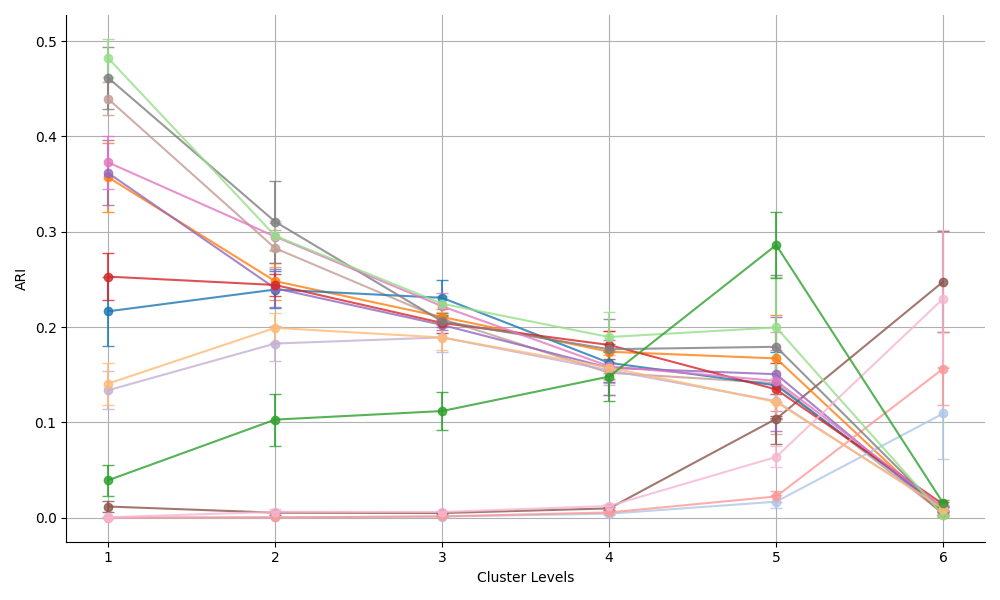
\includegraphics[width=\linewidth]{ARI_plot_None_hierarchy_t1.0_maxsub3_depth5_synonymsNone_noiseNone_random.png}
            \caption*{Deep datasets}
        \end{subfigure}
        \hfill
        \begin{subfigure}[t]{0.49\linewidth}
            \centering
            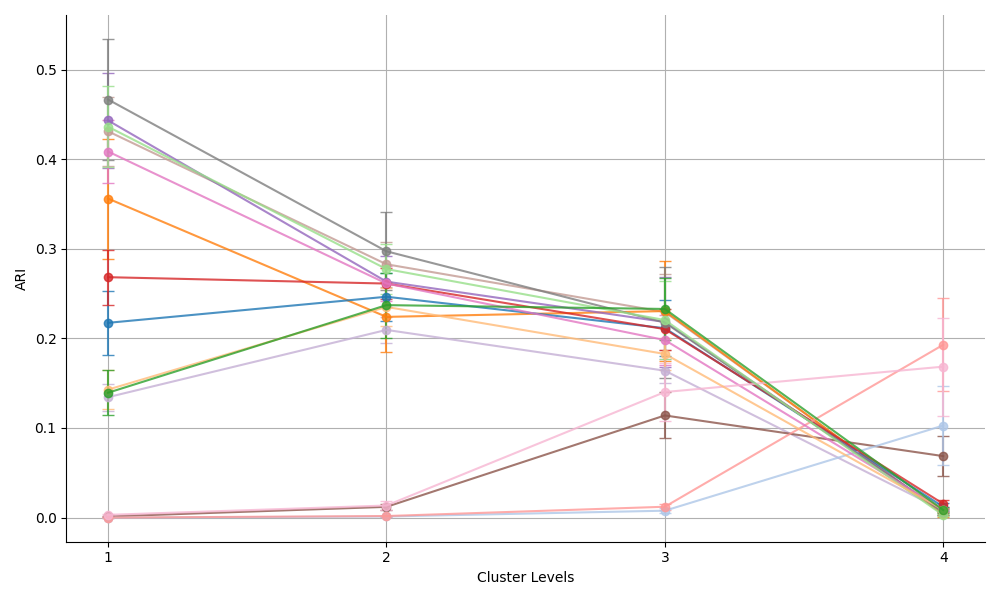
\includegraphics[width=\linewidth]{ARI_plot_None_hierarchy_t1.0_maxsub5_depth3_synonymsNone_noiseNone_random.png}
            \caption*{Shallow datasets}
        \end{subfigure}
    \end{minipage}
    \hfill
    \begin{minipage}[t]{0.25\linewidth}
        \centering
        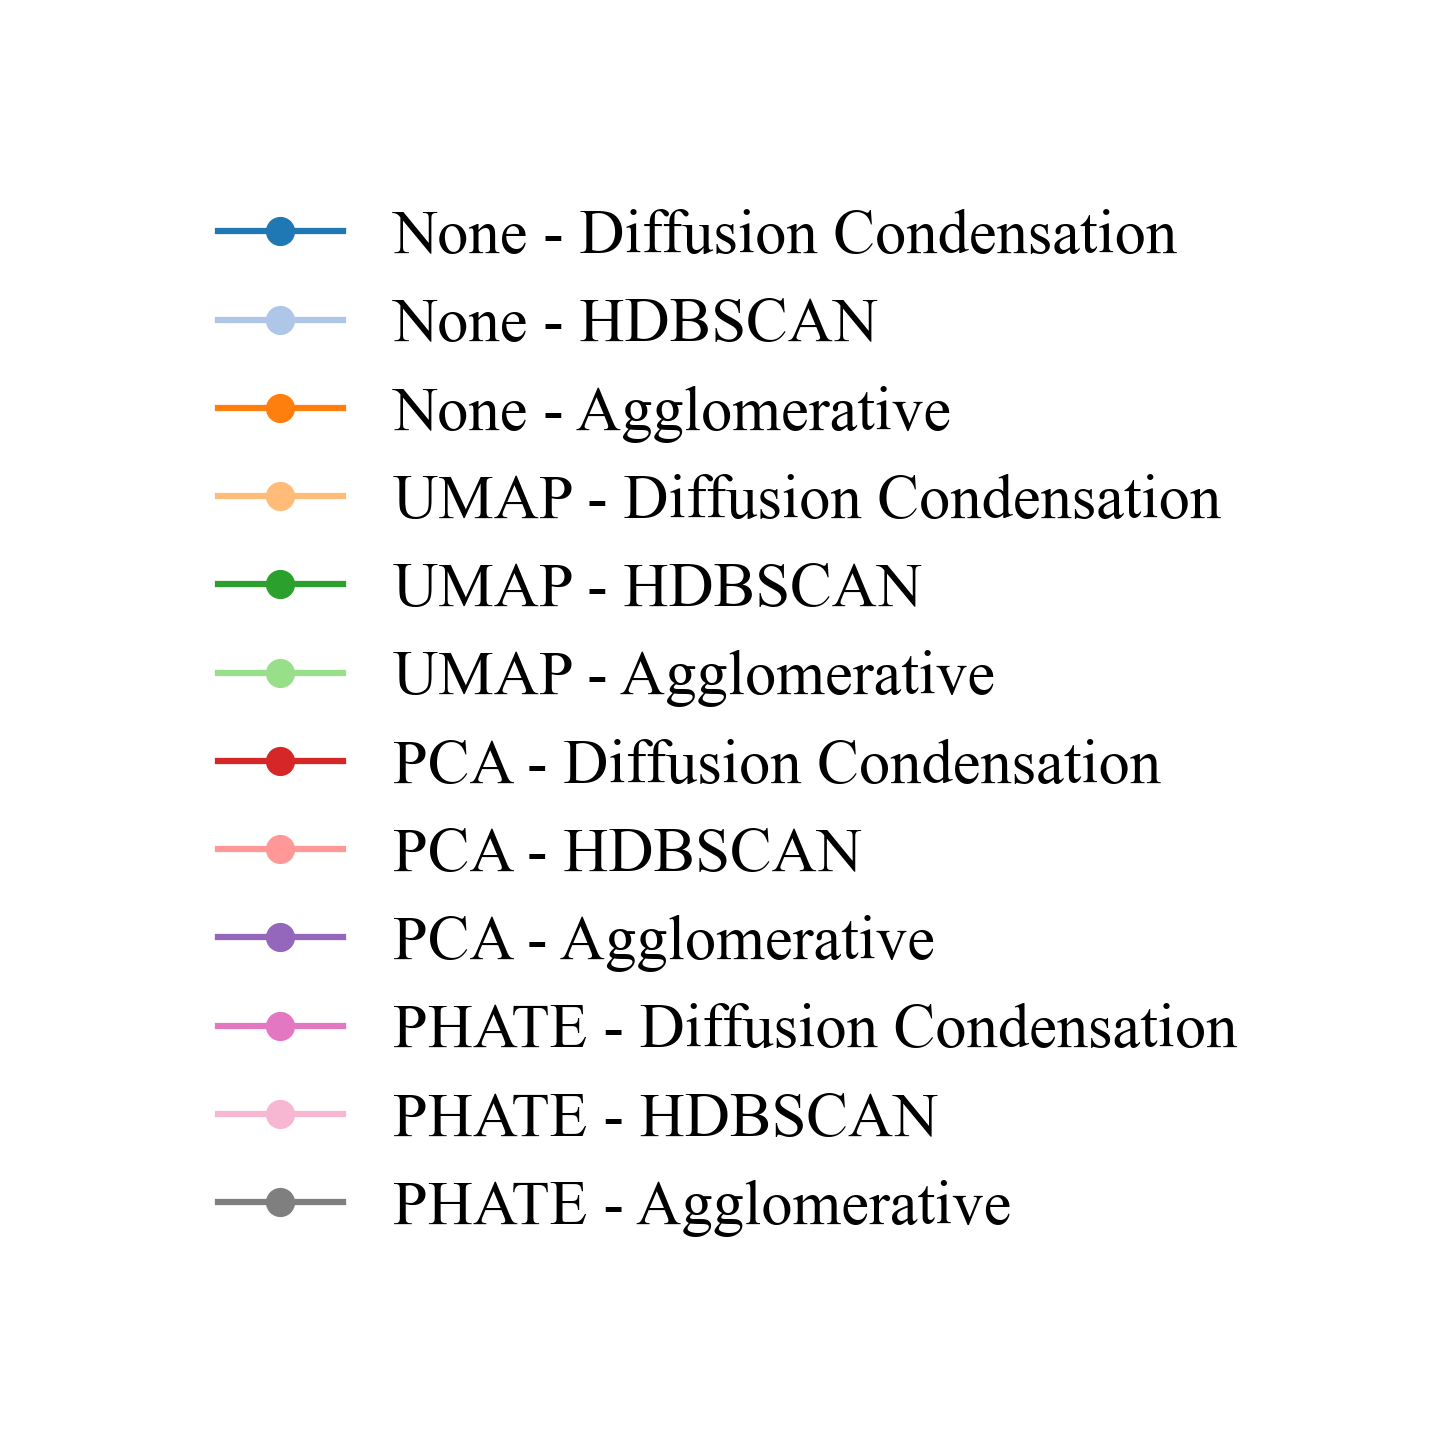
\includegraphics[width=\linewidth]{legend_None_t1.0_maxsub3_depth5_noiseNone_random.png}
    \end{minipage}
    \caption{Line plot of performance at each cluster level averaged across deep and shallow generated datasets. Lower numbers on the x-axis correspond to coarser scales (i.e., fewer clusters). \textit{None} means no dimensionality reduction. Bars represent standard error.}
    \label{fig:ARI-combined}
\end{figure*}

\section{Discussion}
We find that PHATE produces compelling visualizations with desirable features that simultaneously separate classes while preserving mesoscale and global connections. Distal points of the branches of the PHATE embeddings correspond to coarse-scale, archetypal classes, facilitating a straightforward manual identification. 

We find in all cases that PHATE produces more informative visual representations than PCA, UMAP, and t-SNE. We anticipate that this should inform more detailed and robust analyses of textual data, particularly in social science applications.

UMAP coupled with agglomerative clustering generally achieved the strongest performance across the clustering tasks, with consistently higher ARI scores across datasets. PHATE with agglomerative clustering also performed competitively, consistently outperforming PCA though slightly below UMAP on average in many cases. While PHATE visually preserves manifold structure better—particularly where UMAP compresses data into a line or single plane—the quantitative results support both UMAP and PHATE’s overall clustering effectiveness. It should be noted, however, that summary statistics across the clustering levels (i.e., the mean of the medians in Table \ref{tab:pivot_table}) capture only part of the story, and that, numerically, UMAP and PHATE achieve quite comparable results. In many cases, PHATE outperformed UMAP at coarser scales. With hyperparameter tuning, it is entirely possible that one could identify hyperparameter choices that would lead PHATE to outperform the reported results. 

Surprisingly, while satisfactorily recovering fine-scale clusterings in some cases, HDBSCAN consistently failed to produce adequate coarse-scale clusterings. The consistency of this finding suggests careful consideration is warranted when selecting a hierarchical clustering method.

This work focuses on PHATE as an alternative dimensionality reduction technique that emphasizes the preservation of both global and local data structure. Unlike UMAP, which prioritizes local neighborhood preservation and often fragments global trajectories, PHATE explicitly models the continuous diffusion of information across a data manifold, making it better suited for capturing smooth narrative arcs and multiscale semantic hierarchies. PHATE complements existing pipelines, like BERTopic, by offering a new embedding space in which hierarchical relationships and semantic trajectories are more naturally preserved. This approach can either serve as a drop-in replacement for dimensionality reduction in topic modeling workflows or augment existing methods by improving the interpretability and structure of visualizations. Compared to PCA, UMAP, and t-SNE, PHATE provides superior global semantic continuity, which is critical for uncovering latent hierarchies and narrative progressions in textual data. This could be helpful for measuring similarities and differences among graphs with nodes and edges decorated with textual features by utilizing the kernel-based approach suggested in \citet{berijanian2024soft}.

It could be interesting to apply PHATE in a sequential manner for hierarchical clustering in the following sense: Since the branches of the PHATE plots correspond to the most differentiated high-level classes, if one iteratively pruned these branches and reran PHATE on the remaining data, it might be possible to better-recover the nested classes. 


\section{Conclusion}
We have demonstrated that PHATE, a manifold learning technique originally developed for biological data, generalizes effectively to high-dimensional language embeddings. By leveraging both local and global data geometry, PHATE captures semantic and narrative structures in text with greater clarity than conventional techniques such as PCA, UMAP, and t-SNE. A multiscale variant of PHATE further recovers meaningful hierarchical relationships, outperforming standard pipelines in clustering tasks.

Our results show that the structural irregularities common in real-world text—such as dropout analogs, batch effects, and latent hierarchies—are well-handled by PHATE’s diffusion-based approach. Through both synthetic datasets and real policy narratives, we find that PHATE preserves fine- and coarse-grained semantic structure while enhancing interpretability. These findings highlight PHATE’s potential as a valuable tool for unsupervised text analysis, opening new opportunities for its use in natural language processing and computational social science.

\section{Limitations}
While we compared the algorithms on a range of real and synthetic datasets and varied parameters for all methods on equivalent ranges where applicable (i.e., number of components), some methods and parameter choices perform more favorably on particular datasets and at particular scales. To account for this, we report central tendencies (means of medians), choosing the median to reflect an actual outcome while also being less affected by extremely (un)favorable outcomes. The scalability of PHATE is well-documented in \citet{moon2019visualizing}. 

% \section{Acknowledgments}
% Acknowledgments omitted for anonymous review.

\bibliographystyle{acl_natbib}
\bibliography{refs,custom}
\appendix
% \documentclass{article}
% % Define color and JSON style for listings
% \usepackage[preprint]{neurips_2025}
% \usepackage[most]{tcolorbox}
% \usepackage{listings}
% \usepackage{float}
% \usepackage{booktabs}
% \usepackage{array}
% \usepackage{hyperref}
% \usepackage{graphicx}
% \usepackage{xcolor}
% \usepackage{subcaption}
% \usepackage{placeins}

% \definecolor{lightgray}{gray}{0.95}
% \lstdefinestyle{json}{
%   backgroundcolor=\color{lightgray},
%   basicstyle=\ttfamily\small,
%   breaklines=true,
%   frame=single,
%   showstringspaces=false
% }
% \begin{document}

\section{Technical Appendices}
\subsection{Code and Data Availability}
All code and data necessary for replicating experiments can be accessed here: \url{https://anonymous.4open.science/r/phate-for-text-4D7D/README.md}. 
\subsection{Parameter Selection Process}
\label{subsec:parameters}
Parameter selection for both the dimensionality reduction and clustering followed a progressive refinement strategy. We explored a broad range of parameter combinations. Each combination of method and parameters was evaluated on the smaller synthetic datasets to assess baseline performance.

\begin{table*}[ht]
\centering
\caption{Initial parameters for dimensionality reduction and clustering}
\begin{tabular}
{@{}lp{10cm}@{}}
\toprule
\textbf{Method} & \textbf{Parameters} \\ \midrule
UMAP & \texttt{n\_components: [100, 300], min\_dist: [0.05, 0.1, 0.2, 0.3, 0.4, 0.5], n\_neighbors: [5, 10, 15, 25]} \\ \midrule
PCA & \texttt{n\_components: [100, 300]} \\ \midrule
PHATE & \texttt{n\_components: [100, 300], decay: [10, 20, 40], t: [7, 11, auto], knn: [3, 5, 7]} \\ \midrule
HDBSCAN & \texttt{cluster\_selection\_epsilon: [0, 0.1, 0.01, 0.001], cluster\_selection\_method: [eom, leaf]} \\ \midrule
Agglomerative clustering & \texttt{linkage: [ward, average]} \\ \midrule
Diffusion condensation & \texttt{k: [4, 5, 10], t: [3, 10, 30], alpha: [2, 4, 8], bandwidth\_norm: [max, l1]} \\
\bottomrule
\end{tabular}
\end{table*}

% \begin{table}[H]
% \centering
% \caption{Initial parameters for dimensionality reduction and clustering}
% \begin{tabular}{@{}lp{7cm}@{}}
% \toprule
% \textbf{Method} & \textbf{Parameters} \\ \midrule
% UMAP & 
% \begin{tabular}[t]{@{}l@{}}
% \texttt{n\_components: [100, 300],} \\
% \texttt{min\_dist: [0.05, 0.1, 0.2, 0.3, 0.4, 0.5],} \\
% \texttt{n\_neighbors: [5, 10, 15, 25]}
% \end{tabular} \\ \midrule
% PCA & 
% \texttt{n\_components: [100, 300]} \\ \midrule
% PHATE & 
% \begin{tabular}[t]{@{}l@{}}
% \texttt{n\_components: [100, 300], decay: [10, 20, 40],} \\
% \texttt{t: [7, 11, auto], knn: [3, 5, 7]}
% \end{tabular} \\ \midrule
% HDBSCAN & 
% \begin{tabular}[t]{@{}l@{}}
% \texttt{cluster\_selection\_epsilon: [0, 0.1, 0.01, 0.001],} \\
% \texttt{cluster\_selection\_method: [eom, leaf]}
% \end{tabular} \\ \midrule
% Agglomerative clustering & 
% \texttt{linkage: [ward, average]} \\ \midrule
% Diffusion condensation & 
% \begin{tabular}[t]{@{}l@{}}
% \texttt{k: [4, 5, 10], t: [3, 10, 30],} \\
% \texttt{alpha: [2, 4, 8], bandwidth\_norm: [max, l1]}
% \end{tabular} \\
% \bottomrule
% \end{tabular}
% \end{table}

We evaluated performance using both random forest classifiers and simple averaging metrics to identify high-performing parameter configurations. For the random forest we used the parameters as predictors and average ARI as the target. Based on these results, we reduced the search space and standardized the dimensionality parameter $\mathtt{n\_components}$ to values of 100 and 300 across all dimensionality reduction methods.
\begin{table*}[ht]
\centering
\caption{Refined parameters for larger synthetic datasets}
\begin{tabular}{@{}lp{10cm}@{}}
\toprule
\textbf{Method} & \textbf{Parameters} \\ \midrule
UMAP & \texttt{n\_components: [100, 300], min\_dist: [0.05, 0.1], n\_neighbors: [10, 15]} \\ \midrule
PCA & \texttt{n\_components: [100, 300]} \\ \midrule
PHATE & \texttt{n\_components: [100, 300], decay: [20], t: [auto]} \\ \midrule
HDBSCAN & \texttt{cluster\_selection\_epsilon: [0, 0.001], cluster\_selection\_method: [eom]} \\ \midrule
Agglomerative clustering & \texttt{linkage: [ward]} \\ \midrule
Diffusion condensation & \texttt{k: [5, 10], t: [3, 10], alpha: [4], bandwidth\_norm: [max]} \\ 
\bottomrule
\end{tabular}
\end{table*}

Parameters were selected on the basis of best mean performance from the previous step. $\mathtt{n\_components}$ was universally chosen as 300.  
\begin{table*}[ht]
\centering
\caption{Final parameters for largest and real-world datasets}
\begin{tabular}{@{}lp{10cm}@{}}
\toprule
\textbf{Method} & \textbf{Parameters} \\ \midrule
UMAP & \texttt{n\_components: [300], min\_dist: [0.05], n\_neighbors: [10]} \\ \midrule
PCA & \texttt{n\_components: [300]} \\ \midrule
PHATE & \texttt{n\_components: [300], decay: [20], t: [auto]} \\ \midrule
HDBSCAN & \texttt{cluster\_selection\_epsilon: [0], cluster\_selection\_method: [eom]} \\ \midrule
Agglomerative clustering & \texttt{linkage: [ward]} \\ \midrule
Diffusion condensation & \texttt{k: [10], t: [3], alpha: [4], bandwidth\_norm: [max]} \\
\bottomrule
\end{tabular}
\label{tab:final-parameters}
\end{table*}

UMAP parameters selected on the basis of hierarchical clustering did not produce desirable visualizations. % This is partially due to visualizing with the top 2 coordinates with \texttt{n\_components=300}. 
Hence, to ensure a fair visual comparison with PHATE in particular, the second-best configuration of UMAP parameters (Table \ref{tab:UMAP-viz})  were used for the generated data visualizations in the results. %The default parameters had emerged as the second-best configuration via the hierarchical clustering evaluation. This adjustment was made solely for visualization purposes and does not affect the integrity of the main comparative analysis.
In the interest of transparency, we have also included the plots generated using the best-performing parameter set (as listed in Table \ref{tab:final-parameters}) in Figure \ref{fig:UMAP-alt} for reference. For completeness, we also include visualizations of the data sets with default parameter settings for PHATE and UMAP in Figure \ref{fig:default-visuals} (we did not vary PCA or t-SNE  parameters that affect 2-D visualization).  %The fact that the best-performing hierarchical clustering parameters for PHATE also produced informative visualizations speaks to the robustness of the method for visualizing textual data.

\begin{table*}[ht]
\centering
\caption{UMAP parameters used only for generated data visualizations.}
\begin{tabular}{@{}lp{10cm}@{}}
\toprule
\textbf{Method} & \textbf{Parameters} \\ \midrule
UMAP (visualization only) & \texttt{n\_components: [300], min\_dist: [0.1], n\_neighbors: [15]} \\
\bottomrule
\end{tabular}
\label{tab:UMAP-viz}
\end{table*}

\begin{figure*}[ht]
    \centering
    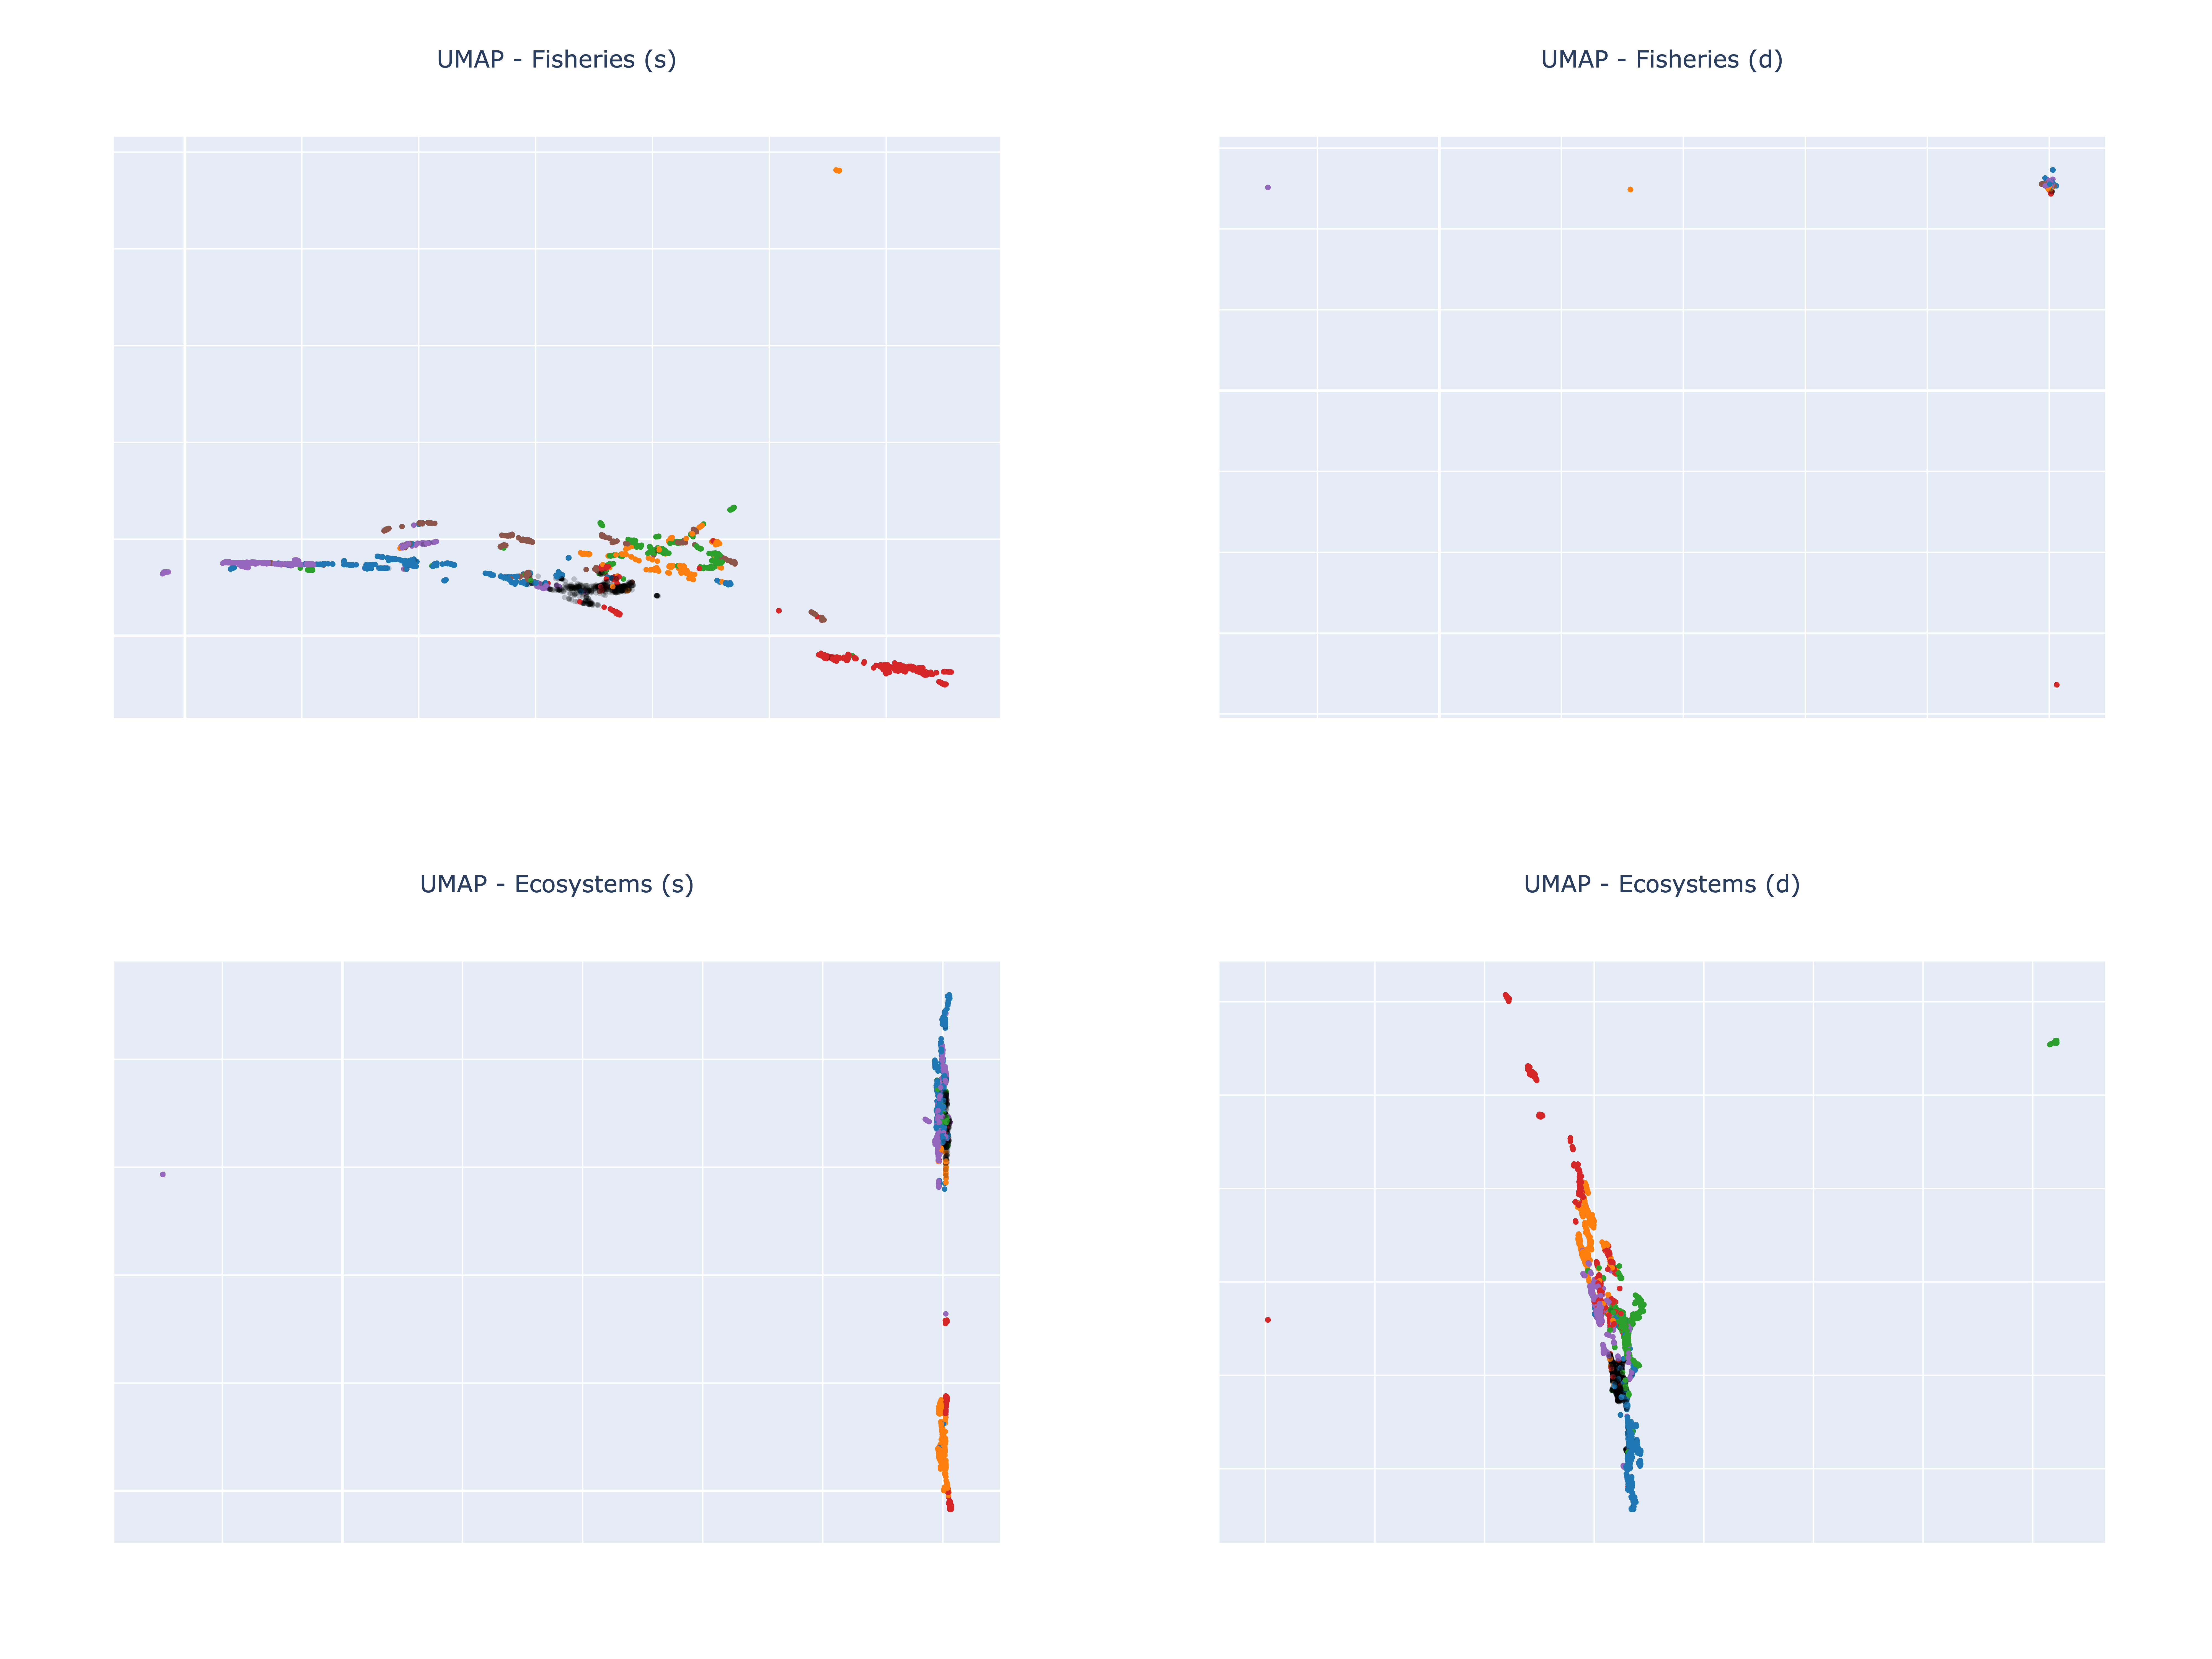
\includegraphics[width=1\linewidth]{UMAP_alternate_params.png}
    \caption{UMAP visualizations of generated data using top-performing clustering parameters}
    \label{fig:UMAP-alt}
\end{figure*}  

\begin{figure*}[ht]
    \centering
    \includegraphics[width=.9\linewidth,keepaspectratio=true]{all_embeddings_subplot_defaults.png}
    \caption{UMAP and PHATE embeddings visuals with default parameters}
    \label{fig:default-visuals}
\end{figure*}  

\subsection{Example GPT Query Prompt and Response}
\subsubsection*{System and user prompt}
In this example, the \textbf{Parent Topic} is the direct parent, while the \textbf{Core Topic} is the highest-level topic in the hierarchy.

% \begin{tcolorbox}[title=System and User Prompt, colback=gray!5, colframe=gray!40!black, boxrule=0.5pt, breakable=unlimited]
\begin{lstlisting}[style=json]
[
  {
    "role": "system",
    "content": "You generate hierarchical topic structures and maintain consistency across responses.
    - Subtopics must be distinct and separate from one another.
    - Subtopics must be more specific than the parent but still general.
    - Each subtopic must be measurable in magnitude (able to increase or decrease, but does not include whether it is an increase or decrease).
    - You have flexibility to generate fewer subtopics if meaningful distinctions become unclear.
    - Subtopics should not describe change itself (e.g., 'fluctuation in X'), but rather be the thing that changes.
    - Subtopics should not merely influence the parent topic but be a sub-example or more specific application of the parent."
  }
]
...
\end{lstlisting}
% \end{tcolorbox}

Expand the given Parent Topic into a list of up to 5 or fewer specific subtopics that:
- Are related to Economic Impact Metrics, especially Economic Impact Metrics.
- Clearly reflect their connection to the Parent Topic and Core Topic through their nature and scope.
- Are Not related to the other core topics: [].
- Much Less related to sibling topics: [].
- Fit within the given theme: Energy, Ecosystems, and Humans.
- Each subtopic should be a subcategory of the parent topic, such that a change in the subtopic implies a change in the broader topic.

Parent Topic: Renewable Energy Investment 
Core Topic: Economic Impact Metrics

Output Format: A JSON list of up to 5 subtopics, e.g.:

["Subtopic 1", "...", "Subtopic 5"]


\subsubsection*{Generated output}

...

% \begin{tcolorbox}[title=Model Output, colback=gray!5, colframe=gray!40!black, boxrule=0.5pt]
\begin{lstlisting}[style=json]
  [
    "Job Creation in Renewable Sector",
    "Capital Expenditure on Green Technologies",
    "Subsidies for Renewable Energy Projects",
    "Grid Infrastructure Upgrades for Renewables",
    "R&D Investment in Renewable Technologies"
  ]
  \end{lstlisting}
  % \end{tcolorbox}
\subsection{Dataset Details}
We evaluated our method on three publicly available datasets, each containing hierarchical categorical labels. Below, we detail the preprocessing, embedding, and clustering procedures applied to each dataset.

\subsubsection*{Amazon Product Reviews}

This dataset is derived from Amazon product reviews. Each entry includes a product \texttt{Title} and three hierarchical category levels (i.e., \texttt{Cat1}, \texttt{Cat2}, \texttt{Cat3}). We used the product title as the input text for embedding. The three category levels served as the hierarchical ground truth for evaluating the clustering quality. This dataset allowed us to analyze how product titles align with categorical hierarchies in a consumer retail context.

\subsubsection*{DBpedia}

For the purposes of embedding and visualization, we processed the text from the train, validation, and test splits. We used the textual description fields as input for embedding and dimensionality reduction. Clustering evaluation was then performed on the test set using the provided hierarchical labels (\texttt{l1}, \texttt{l2}, \texttt{l3}) as the categorical hierarchy.

\subsubsection*{Web of Science}

For each paper in the Web of Science (WOS) corpus, we used the provided keywords as the textual input for embedding and reduction. We then performed clustering on the resulting representations. Hierarchical labels were derived from the \texttt{Domain} and \texttt{area} fields, which represent high-level and mid-level classifications respectively. These served as the ground truth for evaluating the clustering performance.
\subsubsection*{arXiv}

The arXiv dataset contains approximately 30,000 scientific documents constructed from titles and abstracts. Documents were filtered to relevant domains and used to form a unified textual representation. Hierarchical ground truth labels were derived from subject categories at two levels (L1 and L2). Embeddings were generated using \texttt{all-MiniLM-L6-v2} and \texttt{Qwen3-Embedding-0.6B}.

\subsubsection*{RCV1}
The RCV1 dataset consists of news articles annotated with hierarchical topic codes. We used a processed subset where each document combines headline and body text. Ground truth labels were derived from Reuters topic codes, forming a hierarchical structure. Embeddings were generated using both \texttt{all-MiniLM-L6-v2} and \texttt{Qwen3-Embedding-0.6B}, and the same dimensionality reduction and clustering pipeline was applied as in the arXiv experiments.


\subsubsection*{Environmental Protection Agency (EPA)}
Comments were obtained from the federal register through Mirrulations\footnote{https://registry.opendata.aws/mirrulations/}. Comments were filtered to include only those relevant to the EPA. Standard pre-processing steps were applied, including removal of stop-words, HTML tags, and punctuation. Very short comments (<10 characters) were discarded, and long comments (>512 tokens) were truncated using a head-tail strategy (first and last 25\%). Only comments submitted after 2000 were retained. Sentence embeddings were generated using the Sentence-BERT model \texttt{all-MiniLM-L6-v2}.
% Across all datasets, we applied consistent embedding and dimensionality reduction techniques before performing clustering. Hierarchical clustering quality was assessed using the corresponding multi-level categorical labels, with particular emphasis on the test set where applicable.

\subsection{Hardware and runtime environment}
\begin{itemize}
  \item \textbf{Device:} Apple MacBook Pro 16-inch
  \item \textbf{Chip:} Apple M3 Max
  \item \textbf{CPU Cores:} 16-core CPU (12 performance cores, 4 efficiency cores)
  \item \textbf{GPU:} Not used for the majority of experiments
  \item \textbf{RAM:} 64 GB
  \item \textbf{Purpose:} All experiments, including data generation and evaluation, were conducted locally on this machine.
  \item \textbf{Runtime Summary:}
  \begin{itemize}
    \item Data generation tasks were completed in approximately 1 hour for the largest datasets.
    \item The parameter search for generated datasets took under 72 hours in total.
    \item Evaluation on DBpedia completed in 24 hours.
    \item The evaluations on Amazon and Web of Science were completed in less than 6 hours each.
  \end{itemize}
  % \item \textbf{Dataset Evaluation Pipeline:}
  % \begin{itemize}
  %   \item All data sets were embedded using GPT-based representations.
  %   \item Dimensionality reduction was performed using UMAP, PHATE, t-SNE, and PCA.
  %   \item Each reduced data set was clustered using Agglomerative Clustering, HDBSCAN, and Diffusion Condensation.
  %   \item Clustering was also performed on the raw text embeddings of the generated (synthetic) data sets.
  % \end{itemize}
  
\end{itemize}


% \end{document}

\end{document}
